%latex <filename>.tex
%makeindex <filename>.nlo -s nomencl.ist -o <filename>.nls
%latex <filename>.tex

\documentclass[12pt,oneside]{Classes/uitBA}
\usepackage{multicol}
\usepackage[utf8]{vietnam}
\usepackage[utf8]{inputenc}
\newtheorem{theorem}{Định lý}
\newtheorem{definition}{Định nghĩa}
\newtheorem{problem}{Bài toán}
\usepackage{amsmath}
\usepackage{algorithm}% http://ctan.org/pkg/algorithms
\usepackage{algcompatible}% http://ctan.org/pkg/algorithmicx
\usepackage{mathtools,amssymb}

\usepackage{pgfplots}
\pgfplotsset{width=7cm,compat=1.8}

\usepackage{amsmath}
\usepackage{listings}
\usepackage{float}
\usepackage{indentfirst}
%\documentclass{standalone}
\usepackage{pgfplots}
\pgfplotsset{compat=1.3}
%\usepackage{glossaries}
\usepackage{booktabs}
\usepackage{graphicx}
\usepackage{caption}
\usepackage[numbers]{natbib}
\usepackage{notoccite}
\usepackage{nomencl}
\makenomenclature

\usepackage{ifthen}
\renewcommand{\nomgroup}[1]{%
	\item[\bfseries
	\ifthenelse{\equal{#1}{KH}}{Các ký hiệu}{%
			\ifthenelse{\equal{#1}{KN}}{Các khái niệm viết tắt}{}}%
	]}

\ifpdf
\pdfinfo { /Title  (Thesis title)
	/Creator (TeX)
	/Producer (pdfTeX)
	/Author (Nguyen Duc Thang)
	/CreationDate (D:20170110213532)  %format D:YYYYMMDDhhmmss
	/ModDate (D:20170110213532)
	/Subject (KL title)
	/Keywords (Khoa luan)}
\pdfcatalog { /PageMode (/UseOutlines)
	/OpenAction (fitbh)  }
\fi

\university{{\textbf{ĐẠI HỌC THĂNG LONG}}}
\collegeordept{{KHOA HỌC MÁY TÍNH}}  
\degree{}   
\title{{{\Large PHÁT HIỆN CỘNG ĐỒNG TRONG MẠNG TƯƠNG TÁC KÍCH THƯỚC LỚN}}} 
\crest{
\includegraphics[scale=1]{Logo_Thanglong}} 
\supervisor{{TS. TRẦN VĨNH ĐỨC \\}}
\author{{NGUYỄN ĐỨC THẮNG - A22852}}   
\degreedate{HÀ NỘI - 2017} 
\hbadness=10000
\hfuzz=50pt
\usepackage{StyleFiles/watermark}

\onehalfspacing

\begin{document}
	\maketitle
	\setcounter{secnumdepth}{3}
	\setcounter{tocdepth}{3}
	
	\frontmatter % book mode only
	\pagenumbering{roman}
	% 
\begin{dedication}  


\end{dedication}

 
	
\begin{acknowledgements}
	\setlength{\parindent}{5ex}
	Lời đầu tiên, tôi xin gửi lời cảm ơn trân trọng và sâu sắc tới các thầy cô thuộc Bộ môn Tin học - Khoa Toán tin trường Đại học Thăng Long, đã tận tâm truyền đạt những kiến thức quý báu trong quá trình học tập và thực hiện khóa luận này. \par
	
	Đặc biệt, tôi xin gửi lời cảm ơn chân thành và sâu sắc tới TS. Trần Vĩnh Đức, người đã trực tiếp hướng dẫn tận tình và đóng góp những ý kiến quý báu và Ths. Trần Tuấn Toàn đã tạo điều kiện sử dụng phòng máy trong quá trình thực nghiệm khóa luận này. \par
	
	Cuối cùng, tôi xin được gửi lời cảm ơn đến gia đình, người thân và bạn bè của tôi, những người đã ở bên, khuyến khích và động viên trong cuộc sống, học tập.\par
	
	Trong quá trình thực hiện khóa luận của mình, tôi đã có gắng hết sức để tìm hiểu và hoàn thiện một cách tốt nhất. Nhưng với kiến thức và sự hiểu biết còn hạn chế, khóa luận này sẽ không tránh khỏi những thiếu sót, kính mong nhận được những góp ý của các thầy cô, các bạn và những người quan tâm đến khóa luận này.\par
	
\textbf{Tôi xin chân thành cảm ơn!}
	
\begin{multicols}{2}
	\qquad\qquad\quad 
	\columnbreak \\
	\centering{\textit{Sinh viên thực hiện}}
	\par \medskip
	\par \medskip
	\par \medskip
	\par \medskip
	\par \medskip
	\par \medskip
	\par \medskip
	\par \medskip
	\par 
	\centering{\textbf{Nguyễn Đức Thắng}}
\end{multicols}
\end{acknowledgements}
  
	\begin{loicamdoan}
	\setlength{\parindent}{5ex}
	Tôi xin cam đoan đề tài phát hiện cộng đồng trong mạng xã hội lớn, thực hiện dựa trên mô hình BigCLAM và các thuật toán học máy được trình bày trong khóa luận là do tôi thực hiện dưới sự hướng dẫn của TS. Trần Vĩnh Đức.\par 
	
	Tất cả các bài báo, tài liệu, công cụ phần mềm của các tác giả khác được sử dụng trong khóa luận này đều được chỉ dẫn tường minh về nguồn và tác giả trong danh sách tài liệu tham khảo. 
	
\begin{multicols}{2}
	\qquad\qquad\quad 
	\columnbreak \\
	\centering{Hà Nội, ngày 10 tháng 06 năm 2017} \par
	\centering{\textit{Sinh viên thực hiện}}
	\par \medskip
	\par \medskip
	\par \medskip
	\par \medskip
	\par \medskip
	\par \medskip
	\par \medskip
	\par \medskip
	\par 
	\centering{\textbf{Nguyễn Đức Thắng}}
\end{multicols}
\end{loicamdoan}
	 
\begin{abstracts}  
\nomenclature[KN]{BigCLAM}{Cluster Affiliation Model for Big Networks}   
Với sự phát triển nhanh chóng của các cộng đồng mạng kết nối như mạng xã hội Facebook, Twitter, Youtube,\dots hay mạng thương mại điện tử như Amazon, Netfix, Lazada,\dots việc phân tích các mạng này đóng vai trò ngày càng quan trọng, thời sự và được sự quan tâm nghiên cứu thuộc nhiều lĩnh vực như xã hội học, kinh tế, khoa học máy tính,\dots Trong đó bài toán phát hiện cộng đồng trong các mạng tương tác đang là một trong những nội dung nghiên cứu dành được nhiều sự quan tâm từ phía các nhà khoa học. Các nhà khoa học đã đề xuất rất nhiều các phương pháp phát hiện cộng đồng trong mạng tương tác, đặc biệt là các mạng có tính chồng chéo, trong số đó mô hình BigCLAM (Cluster Affiliation Model for Big Networks) được Yang.J và Leskovec.L đề xuất năm 2013 được chứng mình là khá nổi trội trong việc phát hiện cộng đồng chồng chéo trong mạng có kích thước lớn.
\nomenclature[KN]{SNAP}{Stanford Network Analysis Project} 

Đề tài này sẽ đi sâu vào nghiên cứu mô hình BigCLAM và đề xuất một vài phương pháp huấn luyện cũng như phương pháp tối ưu tốc độ huấn luyện. Trong quá trình thực nghiệm khóa luận, phương pháp được cài đặt trên hệ thống tính toán phân tán và sử dụng mạng có kích thước lớn trên trang SNAP\footnote{http://snap.stanford.edu} của Đại học Stanford như Facebook, Amazon, Youtube, \dots

Nội dung của khóa luận gồm 5 chương:

\textbf{Chương 1: Tổng quan về mạng và bài toán phát hiện cộng đồng chồng chéo}. Tại chương này của khóa luận trình một cách khái quát về mô hình mạng tương tác trong thực tế và các bài toán liên quan đặc biệt là bài toán phát hiện cộng đồng. Từ đó thiết lập động lực và mục tiêu của khóa luận này.

\textbf{Chương 2: Cơ sở lý thuyết}. Trong chương này sẽ trình bày chi tiết các khái niệm cơ sở được sử dụng trong khóa luận.

\textbf{Chương 3: Phương pháp phát hiện cộng đồng sử dụng mô hình BigCLAM}. Chương này sẽ trình bày một cách chi tiết về mô hình BigCLAM sử dụng phương pháp cực đại hàm khả dĩ để giải quyết bài toán phát hiện cộng đồng.

\textbf{Chương 4: Cài đặt phương pháp phát hiện cộng đồng sử dụng mô hình BigCLAM trên hệ thống phân tán}. Tại chương này sẽ giới thiệu mô hình tính toán phân tán Apache Hadoop và Apache Spark trong xử lý dữ liệu lớn. Đồng thời đề xuất mô hình cài đặt BigCLAM mới chạy trên hệ thống tính toán phân tán.

\textbf{Chương 5: Kết luận và hướng phát triển}. Đưa ra những kết quả của khóa luận và trình bày phương hướng phát triển sau khóa luận.

\end{abstracts}
 
	\tableofcontents
	\listoffigures
	\listoftables
	\newpage
	\renewcommand{\nomname}{Danh mục ký hiệu và từ viết tắt}
	\addcontentsline{toc}{chapter}{Danh mục ký hiệu và từ viết tắt}
	\addtocontents{toc}{\protect\thispagestyle{empty}}%
	\renewcommand{\nompreamble}{Dưới đây là danh sách các ký hiệu và từ viết tắt đã được sử dụng trong đề tài này.}
	\printnomenclature[1in]
	
	
	\mainmatter  
	\chapter{Tổng quan về mạng tương tác và bài toán phát hiện cộng đồng}\label{chap:c1}
\ifpdf
    \graphicspath{{Chapter1/Chapter1Figs/PNG/}{Chapter1/Chapter1Figs/PDF/}{Chapter1/Chapter1Figs/}}
\else
    \graphicspath{{Chapter1/Chapter1Figs/EPS/}{Chapter1/Chapter1Figs/}}
\fi
\section{Tổng quan về mạng tương tác}

Big Data là một thuật ngữ dùng để chỉ một tập hợp dữ liệu có kích thước lớn và phức tạp mà không thể xử lý trên những công cụ xử lý dữ liệu truyền thống. Thống kê cho thấy, trong hai năm qua khối dữ liệu trên toàn cầu đã chiếm đến $90\%$ lượng dữ liệu số được tạo ra kể từ khi công nghệ số hóa ra đời. Theo dự đoán của các chuyên gia dữ liệu nhận định rằng tốc độ tăng trưởng của dữ liệu là $62\%$ mỗi năm dự đoán đến năm $2020$ chúng ta sẽ có $40+$ exabytes. 

\begin{figure}[h]
	\centering
	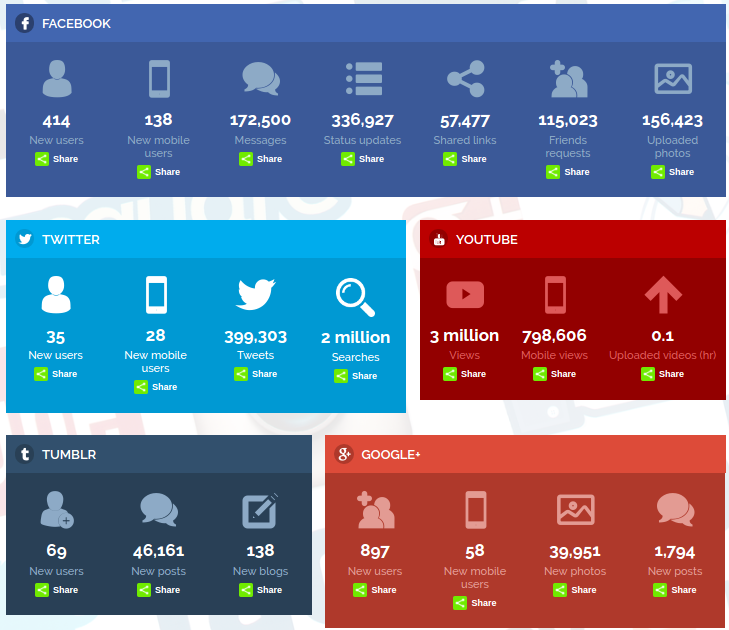
\includegraphics[width=0.6\linewidth]{Chapter1/Chapter1Figs/numberofsocialnetwork}
	\caption{Dữ liệu được sinh ra sau $60s$.}
	\label{fig:numbersocialnetwork}
\end{figure}

Nhìn vào hình \ref{fig:numbersocialnetwork} số liệu (2017)\footnote{http://www.coupofy.com/social-media-in-realtime} cho thấy trung bình cứ $60s$ mạng xã hội Facebook có $336,927$ status updates, $172,150$ mesages, $57,477$ shared links, $115,023$ friends requests,\dots Tương tự như Amazon, Google+, Youtube, Tweeter,\dots đều là những mạng tương tác vô cùng lớn là nơi lưu trữu các thông tin, quan điểm, tính cách, các tương tác giữa các cá thể,\dots Những thông tin này tạo thành đám mây tri thức vô cùng lớn mà chúng ta cần phải khai thác và đưa vào sử dụng. Có thể thấy trong kỷ nguyên số này thì dữ liệu chính là nguồn nhiên liệu vô cùng quan trọng của hầu hết các lĩnh vực. Việt Nam trong thời gian qua cũng đã và đang bắt đầu tiến đến cuộc cách mạng công nghiệp lần thứ tư thúc đẩy quá trình sản xuất thông minh dựa trên các thành tựu về công nghệ thông tin, công nghệ sinh học và công nghệ nano trong đó những bài toán về khai thác và xử lý dữ liệu được đặc biệt quan tâm. Theo lời của GS. Hồ Tú Bảo đã nói "Tới đây hầu hết các công ty đều phải sống dựa vào dữ liệu, ai có nhiều dữ liệu hơn và khai phá được nhiều hơn thì người đó sẽ thắng".

Nhìn nhận lại chúng ta thấy mạng tương tác xuất hiện trong nhiều lĩnh vực như: xã hội học, công nghệ thông tin, khoa học hành vi, toán học, thống kê, y học và nhiều lĩnh vực khác. Mạng tương tác hiện nay được chia ra thành các dạng khác nhau như mạng hiện - ẩn, tĩnh - động, ngoại tuyến - trực tuyến. Chủ yếu dữ liệu mạng tương tác được phân thành hai loại chính như sau:
\begin{itemize}
	\item Nội dung: Chính là các thông tin được lưu trữ trên mạng. Nội dung có thể được hiểu dưới nhiều góc độ khác nhau trong nhiều lĩnh vực như mạng xã hội là các thông tin, trạng khái, bình luận của người sử dụng hay trong mạng sinh học gen chính là các chỗi ADN thông tin. Do đó, kỹ thuật xử lý thường được sử dụng là các phường pháp xử lý văn bản. Tuy nhiên, do tính chất biến động và độ lớn của mạng xã hội hay tính không đầy đủ các thông tin được chia sẻ từ người dùng nên dữ liệu văn bản của mạng xã hội khác với các dữ liệu văn bản truyền thống trước đây. Những bài toán sử dụng dữ liệu này là: phân tích quan điểm người dùng trên mạng xã hội, tím kiếm chủ đề nổi bật trên mạng xã hội,\dots
	\item Cấu trúc: Chính là sự tương tác giữa các cá thể trong mạng. Ví dụ trong mạng xã hội là quan hệ kết bạn, like, share,\dots trong mạng thương mại là quan hệ mua hàng, bán hàng,\dots Cụ thể mạng tương tác được định nghĩa như là một mô hình đồ thị được cấu tạo bởi các đỉnh và các cạnh. Các đỉnh là tập các đối tượng, các cạnh là tập các tương tác giữa các cá thể. Các bài toán sử dụng dữ liệu này là: dự đoán liên kết trong mạng xã hội (được chia thành bốn bài toán con: dự đoán sự tồn tại của liên kết, dự đoán loại liên kết, dự đoán số liên kết, dự đoán số trọng số liên kết), gom nhóm hoặc phân lớp cộng đồng các các thể trong mạng (đây chính là bài toán sẽ được đề cập đến trong khóa luận này),\dots
\end{itemize}
\section{Bài toán phát hiện cộng đồng}
Theo định nghĩa của trên trang Oxford English Dictionary (2017)\footnote{https://en.oxforddictionaries.com/definition/community} thì từ "Communities: A group of people living in the same place or having a particular characteristic in common.". Có thể hiểu, cộng đồng là một nhóm các cá thể trong mạng có những tính chất tương tự nhau và cùng đóng một vai trò trong mạng. Chúng ta có ánh xạ khái niệm cộng đồng trong các mạng tương tác thường thấy như:
\begin{itemize}
	\item Mạng xã hội là một trong những ví dụ điển hình của đồ thị các cộng đồng. Con người có xu hướng kết nối với nhau lại với nhau, hình thành các nhóm (cộng đồng) trong cùng một môi trường làm việc, gia đình, bạn bè, sở thích,\dots
	\item Nghiên cứu y sinh học: Tương tác giữa các protein trong cùng một mô-đun (cộng đồng) sẽ có tính nổi trội hơn.
	\item Hệ khuyến nghị: Khách hàng có thể mua các sản phẩm từ nhóm các sản phẩm có liên quan đến nhau.
	\item \dots
\end{itemize}
 Như vậy nếu các protein, con người, hàng hóa là các tác nhân trong mạng thì các mô-đun, nhóm người dùng hay nhóm sản phẩm chính là các cộng đồng. Và nếu chúng ta phát hiện ra những cộng đồng tiềm năng này cho phép tạo ra nhưng giải pháp tốt nhất về chiến lượng kinh doanh, chữa ung thư, tăng năng suất bán hàng, điều tra tâm lý,\dots Hình\ref{fig:community1} là một ví dụ đơn giản của một mạng tương tác với ba cộng đồng. Dưới đây là phát biểu bài toán phát hiện cộng đồng trong toán học: 
 \nomenclature[KH]{$\mathcal{V}$}{Tập đỉnh}    
 \nomenclature[KH]{$\mathcal{E}$}{Tập cạnh}     
 \nomenclature[KH]{$G(\mathcal{V},\mathcal{E})$}{Đồ thị có $\mathcal{V}$ đỉnh và $\mathcal{E}$ cạnh}
  \nomenclature[KH]{$\mathcal{K}$}{Số cộng đồng}
  \nomenclature[KH]{$\mathcal{K}$}{Số cộng đồng}
  \nomenclature[KH]{$\mathcal{C}$}{Tập cộng đồng}    
 \begin{problem}(Phát hiện cộng đồng trong mạng)\label{def:ncdd1}
 	
 	Cho một đồ thị $G(\mathcal{V},\mathcal{E})$, chúng ta cần khám phá và phát hiện các cộng đồng $C_1,C_2,\dots,C_k$ với $\mathcal{K} \in {\mathcal{C}}$ là số lượng cộng đồng. Trong đó mỗi cộng đồng $C_i \subseteq \mathcal{V}$.
 \end{problem}
 
 Nếu ta thêm một ràng buộc trong bài toán là các $C_i$ là riêng biệt không có sự chồng chéo giữa chúng tức $C_i \cap C_j = \varnothing$, thì ta sẽ có một khái niệm mới cho bài toán \ref{def:ncdd1} là phát hiện cộng đồng không có sự chồng chéo (non-overlapping community detection). Ngược lại, bài toán khóa luận này đề cập đến chính là phát hiện cộng đồng ở đó $C_i$ có khả năng chồng chéo (overlapping community detection).
 
 Hay nói cách khác, phát hiện cộng đồng mạng hay có thể hiểu là việc phân cụm các đỉnh trong một mạng sử dụng cấu trúc mạng kết nối. Và $\mathcal{K}$ ở đây chính là số cộng đồng được ước lượng là tốt nhất.
 
 
\begin{figure}[h]
	\centering
	\begin{minipage}[b]{0.4\textwidth}
		\centering
		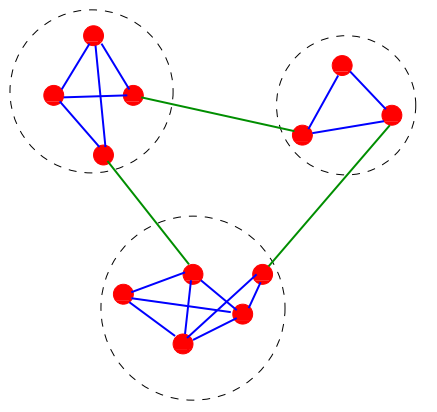
\includegraphics[width=1\linewidth]{Chapter1/Chapter1Figs/community-1}
		\caption{Một mạng tương tác (đồ thị) đơn giản với ba cộng đồng.}
		\label{fig:community1}
	\end{minipage}
	\begin{minipage}[b]{0.58\textwidth}
		\centering
		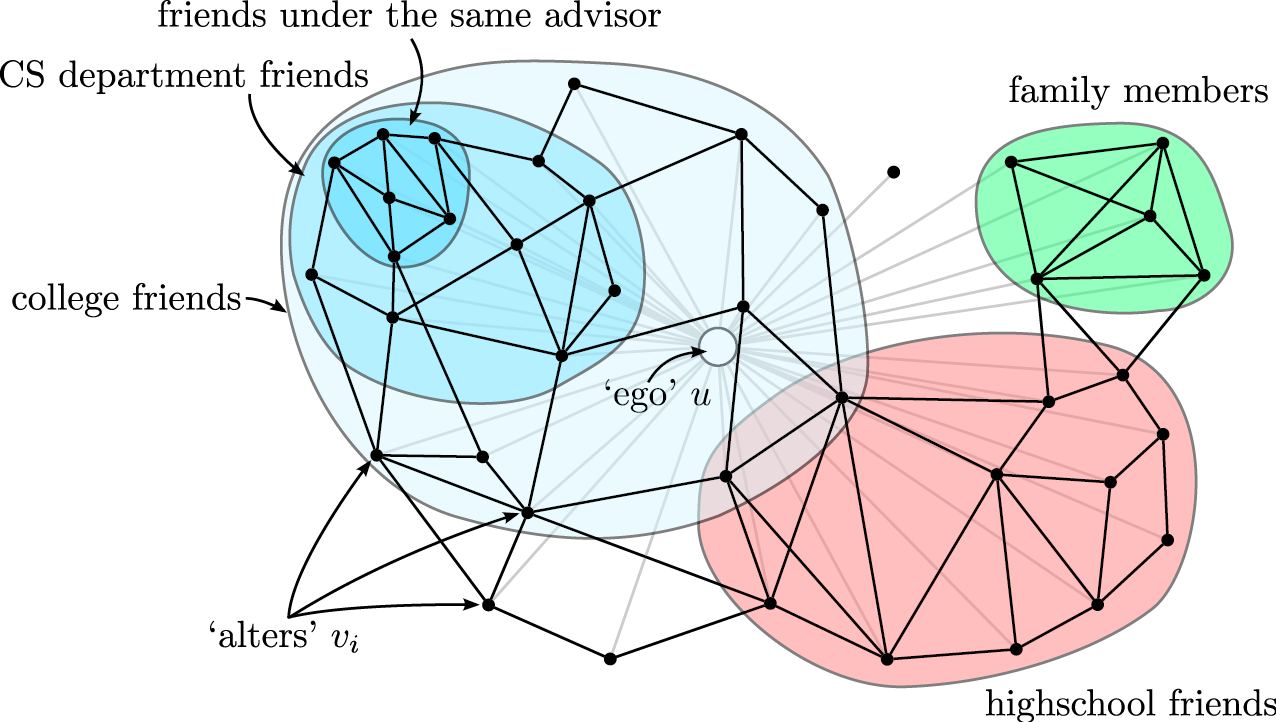
\includegraphics[width=1\linewidth]{Chapter1/Chapter1Figs/overlappingcommunity}
		\caption{Mô tả các cộng đồng trong mạng mạng cá nhân (egonetwork) của một sinh viên Đại học Stanford}
		\label{fig:overlapcommunity}
	\end{minipage}    
\end{figure}

Thực tế hầu như các cộng đồng giàu tính chồng chéo (giao nhau) hoặc là tập con của một cộng đồng khác. Có thể thấy rõ trong mạng xã hội, hình \ref{fig:overlapcommunity} là một kết quả của McAuley and
Leskovec [2012] \cite{DBLP2journals2corr2abs2121028182} cho thấy trong mạng cá nhân của sinh viên này có rất nhiều các cộng đồng khác nhau như family members, highschool fiends, college friends,\dots Và những cộng đồng này đều có tính chồng chéo và có cả những cộng đồng là con của một cộng đồng khác. Vì vậy bài toán phát hiện cộng đồng trong các mạng có đầy đủ cả ba loại cộng đồng như hình \ref{fig:typeofcommunity} là một bài toán khó trong khi sự bủng nổ về kích thước và độ phức tạp của các mạng tăng theo từng phút làm cho bài toán này càng trở lên khó khăn.

\begin{figure}[h]
	\centering
	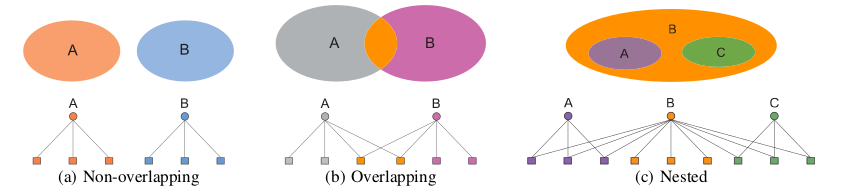
\includegraphics[width=\linewidth]{Chapter1/Chapter1Figs/typeofcommunity}
	\caption{Các loại cộng đồng mà trong mạng tương tác có thể có}
	\label{fig:typeofcommunity}
\end{figure}

Với tiềm năng đầy giá trị của bài toán cũng như những thách thức của bài toán đặt ra, chính là động lực để tôi chọn và thực hiện khóa luận này. Đề tài giải quyết bài toán phát hiện cộng đồng trong các mạng tương tác có kích thước lớn có tính không chồng chéo, chồng chéo và lồng (chứa) nhau trong thời gian cho phép. Trong các chương tiếp theo của khóa luận, tôi sẽ trình bày chi tiết giải quyết bài toán dựa trên mô hình BigCLAM được đề xuất bởi Yang and
Leskovec [2013] \cite{yang2013overlapping} kết hợp với một số phương pháp huấn luyện chạy trên hệ thống tính toán lưới.

\section{Một số nghiên cứu}
Bài toán phát hiện cộng đồng nhận được sự quan tâm từ rất sớm, và có rất nhiều phương pháp giải quyết bài toán \ref{def:ncdd1} có kết quả khá tốt. Tuy nhiên mỗi phương pháp đều có những khuyết điểm, thường khồng phù hợp các mạng có kích thước lớn hiện nay hoặc tỏ ra không vượt trội khi kích thước mạng tăng lên từng giây với thực tế.

\subsection{Phương pháp Girvan-Newman}
Phát hiện cộng đồng dựa trên việc tìm cạnh nối giữa các cộng đồng. Thuật toán này dựa trên quan niệm cho rằng khi các cộng đồng được gắn kết với nhau thì đường đi giữa các cộng đồng này đến cộng đồng khác sẽ đi qua các cạnh nối giữa chúng với tần suất cao. Điểm quan trọng nhất của phương pháp là xây dựng cộng đồng bằng cách loại bỏ dần dần các cạnh nói từ đồ thị ban đầu. Phương pháp này lần đầu tiên được đề xuất bởi Freeman. Theo Freeman, các cạnh được coi là cạnh có số lượng con đường ngắn nhất giữa các cặp đỉnh khác nhau chạy qua nó. Cạnh nối có ảnh hưởng rất lớn đến dòng chảy của thông tin giữa các nút khác, đặc biệt là trong trường hợp thông tin lưu truyền trong mạng chủ yếu theo con đường ngắn nhất. Phương pháp điển hình nhất trong sử dụng tính chất này là phương pháp Girvan-Newman của Newman [2004] \cite{newman2004fast}. Về cơ bản phương pháp Girvan-Newman được thực hiện theo các bước sau:
\begin{enumerate}
	\item Tính độ đo trung gian cho tất cả các cạnh trong mạng;
	\item Hủy bỏ các cạnh có độ trung gian cao nhất;
	\item Tính lại độ trung gian cho tất cả các cạnh bị ảnh hưởng theo các cạnh đã loại bỏ;
	\item Lặp tại từ bước 2 cho đến khi không con các cạnh trung gian ta sẽ có cộng đồng.
\end{enumerate}

\begin{figure}[H]
	\centering
	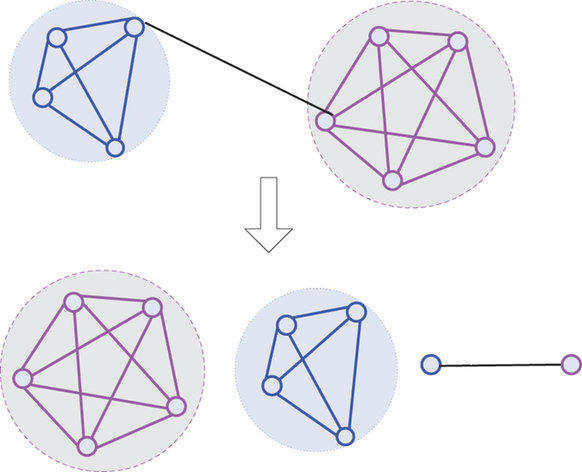
\includegraphics[width=0.5\linewidth]{Chapter1/Chapter1Figs/girvannewman}
	\caption{Minh họa phương pháp Girvan-Newman}
	\label{fig:girvannewman}
\end{figure}
Thuật toán Girvan-Newman khá đơn giản, dễ hiểu và có những kết quả tương đổi tốt trong nhiều trường hợp, mặc dù vậy nó vẫn gặp phải một số nhược điểm:
\begin{enumerate}
	\item Việc tính lại toàn bộ độ trung gian sau mỗi lần loại bỏ các cạnh có độ trung gian cao nhất. Như vậy khiến cho độ phức tạp của thuật toán rất lớn $O(m\times n)$ cho mỗi lần lặp với $m$ là số cạnh và $n$ là số đỉnh. Tổng thời gian chạy thuật toán là $O(m^n\times n)$, trường hợp xấu nhất, mỗi đỉnh là một cộng đồng thì độ phức tạp là $O(m^3)$. Như vậy dường như rất khó khả thi khi chạy trên mạng có kích thước lớn và phức tạp.
	\item Với phương pháp này thì toàn bộ cộng đồng thu được đều riêng biệt. Do vậy không thể làm việc hiệu quả trên mạng có các cộng đồng chồng chéo.
\end{enumerate}

\subsection{Phương pháp CONGA}
\nomenclature[KN]{CONGA}{Cluster Overlap Newman Girvan Algorithm}
Phương pháp CONGA viết tắt của từ Cluster Overlap Newman Girvan Algorithm là một phương pháp nâng cấp của phương pháp Girvan-Newman nhằm khắc phục nhược điểm không phát hiện được các cộng đồng chồng chéo nhau của thuật toán cũ. Các đỉnh sẽ được nhân bản hoặc gộp lại dựa vào một độ đo nhằm tính số cộng đồng mà đỉnh đó thuộc. Gregory [2007] \cite{gregory2007algorithm} đã đề xuất một độ đo đó được gọi là độ trung gian phân chia của đỉnh là số đường đi ngắn nhất mà chạy hai phần của đỉnh sau khi được phân chia. Như vậy với sự nâng cấp này phương pháp CONGA đã giải quyết được vấn đề chồng chéo cộng đồng, tuy nhiên vẫn tồn tại nhược điểm của phương pháp Girvan-Newman vẫn có độ phực tạp tính toán lớn.
\begin{figure}[H]
	\centering
	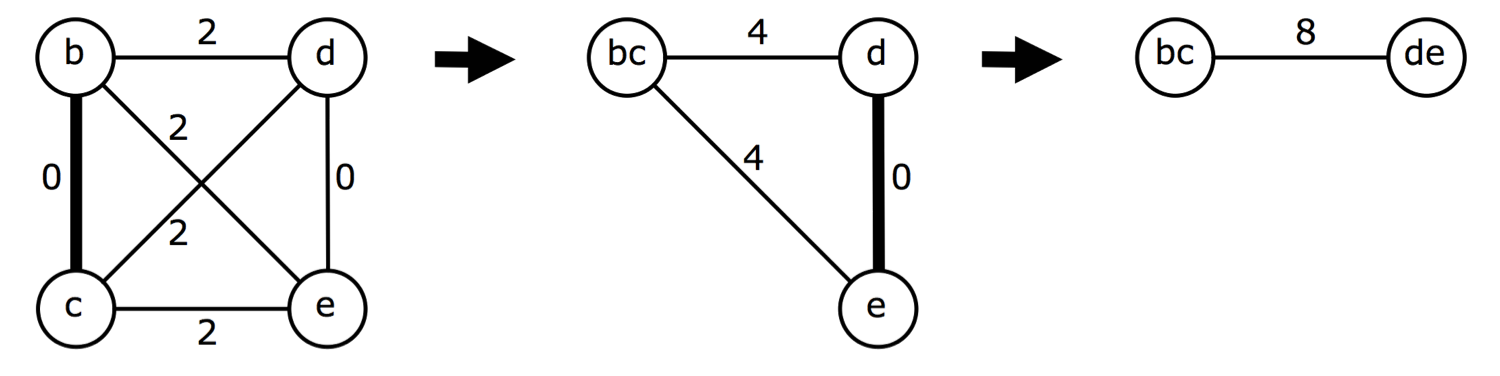
\includegraphics[width=0.8\linewidth]{Chapter1/Chapter1Figs/CONGA}
	\caption{Minh họa phương pháp CONGA}
	\label{fig:conga}
\end{figure}
\subsection{Affiliation Graph Model (AGM)}
\nomenclature[KN]{AGM}{Affiliation graph model}
\nomenclature[KH]{$M$}{Cạnh liên hết các đỉnh với các cộng đồng}
\nomenclature[KH]{$B(\mathcal{V},\mathcal{C},M)$}{Đồ thị hai phần thể hiện mô hình AGM}    
AGM được giới thiệu bởi Yang and Leskovec [2012] \cite{yang2012community} là mô hình xác suất xây dựng dựa trên một đồ thị hai phần (bigraph) $B(\mathcal{V},\mathcal{C},M)$ phần thứ nhất của đồ thị là các đỉnh $\mathcal{V}$ của mạng phần thứ 2 là các đỉnh định danh cho các cộng đồng trong mạng $\mathcal{C}$ mỗi cộng đồng sẽ được gắn với một xác suất $p_A$ kết nối giữa cộng đồng với các đỉnh được thể hiện qua cạnh nối $M$ giữa hai phần của đồ thị. AGM có khả năng phát hiện cộng đồng có tính chồng chéo không chồng chéo và lồng nhau trên mạng có kích thước lớn tương đối hiệu quả. Hình \ref{fig:agm} sẽ minh họa cho mô hình.

\nomenclature[KH]{$p_A$}{Xác suất của một cộng đồng} 

Mục tiêu của phương pháp phát hiện cộng đồng trên mô hình AGM là tìm  $\theta = B(\mathcal{V},\mathcal{C},M,\{p_c\})$:
\begin{equation}\label{ct:agm}
\arg \max_{B(\mathcal{V},\mathcal{C},M,\{p_c\})}{ \prod_{(u,v)\in \mathcal{E}}{p(u,v)}\prod_{(u,v)\notin \mathcal{E}}{(1-p(u,v))}}
\end{equation}
\begin{figure}[H]
	\centering
	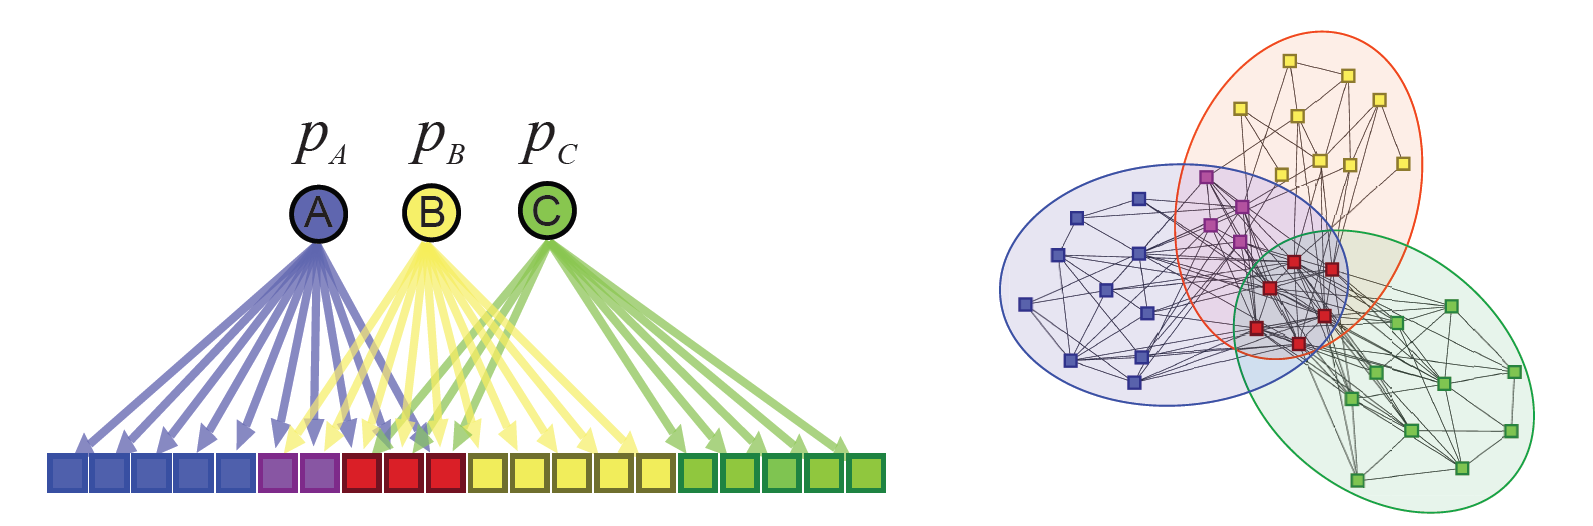
\includegraphics[width=0.8\linewidth]{Chapter1/Chapter1Figs/agm_g}
	\caption{Minh họa mô hình AGM}
	\label{fig:agm}
\end{figure}
Tuy nhiên, theo tác giả để tìm tìm được $B(\mathcal{V},\mathcal{C},M,\{p_c\})$ theo công thức \ref{ct:agm} không hệ đơn giản.

\subsection{Non-negative Matrix Factorization}
\nomenclature[KN]{NMF}{Non-negative Matrix Factorization} 
Non-negative Matrix Factorization (NMF) hay còn gọi phân tích tích matrix không âm thành nhân tử là một kỹ thuật được sử dụng phổ biến giải quyết các bài toán học máy (machine learning), học nhiều tầng (deep learning), hệ khuyến nghị (recommendation system),\dots Trong bài toán phát hiện cộng đồng, NMF tỏ ra khá vượt trội so với các phương pháp khác.

Trong khóa luận này, có đề cập đến mô hình BigCLAM của Yang and Leskovec [2013] \cite{yang2013overlapping} một sự nâng cấp từ mô hình AGM xây dựng dựa trên phương pháp NMF không chỉ trong bài phát hiện cộng đồng chồng chéo mà còn phát hiện được các cộng đồng không chồng chéo và cộng đồng lồng nhau với kết quả vượt trội hơn rất nhiều so với AGM. Mô hình BigCLAM xây dựng một đồ thị hai phần (bipartite graph) giống như AGM phần thứ nhất của đồ thị là các nốt định danh cho các cộng đồng trong mạng phần còn lại là các đỉnh của mạng và cạnh nối giữa các các hai phần của đồ thị chính là độ đo liên kết của các đỉnh trong mạng với các cộng đồng được biểu diễn thành vector. Chi tiết mô hình sẽ được trình bày chi tiết trong chương \ref{chap:c3}.
	\chapter{Cơ sở lý thuyết}\label{chap:c2}
\ifpdf
    \graphicspath{{Chapter2/Chapter2Figs/PNG/}{Chapter2/Chapter2Figs/PDF/}{Chapter2/Chapter2Figs/}}
\else
    \graphicspath{{Chapter2/Chapter2Figs/EPS/}{Chapter2/Chapter2Figs/}}
\fi
Trong chương này, tôi xin trình bày chi tiết các khái niệm cơ bản, thuật ngữ và các ký hiệu được sử dụng trong khóa luận. Tiếp theo, tôi sẽ đề cập đến một số nghiên cứu liên quan đến bài toán phát hiện cộng đồng.

\section{Vector và matrix}

Đầu tiên, tôi sẽ trình bày hai khái niệm cũng như các ký hiệu của vector và matrix không âm. Đây là hai khái niệm quan trọng được sử dụng để thể hiện độ mạnh của các đối tượng, cá thể (đỉnh) trong một cộng đồng trong chương \ref{chap:c3} và \ref{chap:c4}. Dưới đây là nghĩa \ref{df:vectormatrix}:

\begin{definition}(Vector và matrix không âm)\label{df:vectormatrix}
	
	Một vector $\textbf{v} = (v_i) \in \mathbb{R}^n$ là một vector không âm nếu tất cả các phần tử trong $v$ là không âm.($v_i \geq 0$ $\forall i \in \{1, \dots, n\}$)
	
	Tương tự, một matrix $F = (F_{ij}) \in \mathbb{R}^{n \times m}$ là không âm nếu mọi phần tử trong $F$ là không âm. ($F_{ij} \geq 0$ $\forall i \in \{1,\dots, n\}, j \in \{1,\dots, m\} $)
\end{definition}

\section{Lý thuyết đồ thị}
Trong mục này, tôi sẽ cung cấp một số định nghĩa về lý thuyết đồ thị được sử dụng trong chương \ref{chap:c3} và \ref{chap:c4}.

Về cơ bản thì mạng tương tác thường được biểu diễn như một đồ thị $G(\mathcal{V},\mathcal{E})$ gồm $\mathcal{V}$ là tập các đỉnh, và $\mathcal{E}$ là tập các cặp không có thứ tự gồm hai phần tử khác nhau của $\mathcal{V}$ gọi là tập cạnh. Chúng ta thường sử dụng hai thuật ngữ nốt (node) và đỉnh (vertex) để ám chỉ cho $\mathcal{V}$ và cạnh (edge) và liên kết (link) để ám chỉ cho $\mathcal{E}$. Ngoài ra chúng còn được biểu diễn thông qua một ma trận kề (adjacency matrix) được phát biểu qua định nghĩa \ref{dn:matrixke}:
\nomenclature[KH]{$A$}{Matrix kề của đồ thị $G(\mathcal{V},\mathcal{E})$ }
\begin{definition}(Matrix kề cho một đồ thị vô hướng)\label{dn:matrixke}
	
	Cho đồ thị $G = G(\mathcal{V},\mathcal{E})$ là đồ thị vô hướng, một matrix $A = (A_{ij}) \in  \mathbb{R}^{|\mathcal{V}|\times|\mathcal{V}|} (i,j \in \mathcal{V})$ được gọi là matrix kề của $G$ nếu:
	\begin{equation}
		A_{ij} = \left\{
		\begin{array}{cc}
		1 & if (i,j) \in \mathcal{E}\\
		0 & otherwise
		\end{array}
		\right.
	\end{equation}
\end{definition}

Trong lý thuyết đồ thị chúng ta sẽ sử dụng một số tính chất quan trọng để xây dựng mô hình phân chia đồ thị thành các đồ thị con ở đó số liên kết (cạnh) giữa chúng là nhỏ nhất và sự liên kết giứa các cá thể trong mỗi đồ thị con là lớn nhất. Việc phân chia đồ thị thành các đồ thị con như vậy vô cùng thuận lợi cho việc khởi tạo đầu vào cho phương pháp phát hiện cộng đồng được trình bày trong chương \ref{chap:c3}. Ta có định nghĩa \ref{df:dodan} được đề xuất bởi Gleich and
Seshadhri [2011] \cite{DBLP:journals/corr/abs-1112-0031}

\nomenclature[KH]{$\varphi(\mathcal{S})$}{Độ dẫn của một đồ thị con $\mathcal{S}$}
\nomenclature[KH]{$\mathcal{A}(\mathcal{S})$}{Tổng số bậc bên trong mỗi đồ thị con $\matchal{S}$}
\begin{definition}(Độ dẫn của một đồ thị con trong đồ thị vô hướng)\label{df:dodan}
	
	Cho đồ thị $G = G(\mathcal{V},\mathcal{E})$ là đồ thị vô hướng, $A = (A_{ij})$ là một matrix kề của $G$. $\mathcal{S} \subseteq \mathcal{V}$ là một tập đỉnh con trong đồ thị $G$, và $\bar{\mathcal{S}} = \mathcal{V} \setminus \mathcal{S}$ là tập đỉnh còn lại của đồ thi. Độ dẫn của $\mathcal{S}$ là:
	\begin{equation}
		\varphi(\mathcal{S}) = \dfrac{\sum_{i \in \mathcal{S},j \notin \mathcal{S}{A_{ij}}}}{min(\mathcal{A}(\mathcal{S}),\mathcal{A}(\bar{\mathcal{S}}))}
	\end{equation}
	Trong đó $\mathcal{A}(\mathcal{S}) = \sum_{i \in \mathcal{S}}\sum_{j \in \mathcal{V}}A_{ij}$
\end{definition}
Ta có thể coi $\varphi(\mathcal{S})$ là độ dẫn của các cạnh từ các đỉnh trong $\mathcal{S}$ đến các đỉnh bên ngoài $\mathcal{S}$.


Trong khóa luận này, tôi có sử dụng ba khái niệm là đỉnh lần cận, vùng lân cận và vùng lân cận địa phương nhỏ nhất được trình bày trong định nghĩa \ref{df:dinhlancan}
\nomenclature[KH]{$\mathcal{N}(u)$}{Đỉnh lân cận của đỉnh $u$}
\nomenclature[KH]{$N(u)$}{Vùng lân cận của đỉnh $u$}
\begin{definition}(Đỉnh lân cận,vùng lân cận và vùng lân cận địa phương nhỏ nhất)\label{df:dinhlancan}
	Cho đồ thị $G = G(\mathcal{V},\mathcal{E})$ ta có:
	
	$\mathcal{N}(u) = \{v : v \in \mathcal{V}, (u,v) \in \mathcal{E}\}$ là tập các đỉnh lân cận với $u$.
	
	$N(u) = \{u\} \cup \mathcal{N}(u)$ là vùng chứa các đỉnh lân cận của $u$. 
	
	Và một $N(u)$ được gọi là vùng lân cận địa phương nhỏ nhất nếu nó có độ dẫn nhỏ hơn trong tất cả $N(v), v \in \mathcal{N}(u)$. Tức $\varphi(N(u)) \leq \varphi(N(v)), \forall v \in \mathcal{N}(u)$.
\end{definition}

Dưới đây sẽ là một vài khái niệm trong lý thuyết đồ thị được nhắc đến trong khóa luận:
\begin{itemize} 
	\item \textbf{Đồ thị hai phần}: hay còn được gọi là đồ thị phân đôi. Đồ thị $G(\mathcal{V},\mathcal{E})$ là một đồ thị phân đôi, nếu các đỉnh trong tập đỉnh $\mathcal{V}$ có thể chia thành hai tập không giao nhau $\mathcal{V}_1$, $\mathcal{V}_2$ thỏa mãn không có cạnh nối giữa đỉnh bất kỳ thuộc cùng một tập.
	\item \textbf{Đồ thị có hướng và vô hướng}: còn được gọi là đồ thị có hướng và đồ thị vô hướng. Đồ thị $G(\mathcal{V},\mathcal{E})$ là đồ thị vô hướng, nếu $\forall(u,v) \in \mathcal{E} \Leftrightarrow (v,u) \in \mathcal{E}$, các cạnh là các cặp cạnh không có thứ tự của các đỉnh. Nếu các cạnh là các cặp cạnh có thứ tự, ví dụ $(u,v) \in \mathcal{E}$ không nhất thiết $(v,u) \in \mathcal{E})$, thì đồ thị $G(\mathcal{V},\mathcal{E})$ là đồ thị có hướng.
	%\item \textbf{Connected component}: hay còn được gọi là thành phần liên thông. Đối với đồ thị vô hướng $G(\mathcal{V},\mathcal{E})$ gọi là liên thông nếu luôn tồn tại đường đi giữa mọi cặp đỉnh phân biệt của đồ thị. Đối với $G(\mathcal{V},\mathcal{E})$ là đồ thị có hướng gọi lầ liên thông mạnh nếu luôn tồn tại đường đi giữa hai đỉnh bất kỳ của đồ thị, $G(\mathcal{V},\mathcal{E})$ gọi là liên thông yếu nếu có đường đi giữa hai đỉnh bất kỳ của đồ thị vô hướng nền. Vô hướng nền là loại bỏ các hướng của đồ thị. 
	%\item \textbf{Induced subgraph}: được gọi là đồ thị con dẫn xuất. Đồ thị con $G_s(\mathcal{V}_s,\mathcal{E}_s)$ của $G(\mathcal{V},\mathcal{E})$ được coi là dẫn xuất nếu $\mathcal{V}_s \subset \mathcal{V}$ và $\mathcal{E}_s = \{(u,v)\in \mathcal{E}: u,v \in \mathcal{V}_s\}$.
	%\item \textbf{Node degree}: Trong đồ thị có hướng, chúng ta cần phân biệt bậc vào (in-degree) ký hiệu là $d_{in}{(u)}$ bằng số cạnh liên thuộc đi dến $u$ và bậc ra (out-degree) $d_{out}{(u)}$ chính bằng số cạnh liên thuộc đi ra từ $u$. Với đồ thị vô hướng, đỉnh $u$ có bậc ký hiệu là $d(u) = d_{in}{(u)} =d_{out}{(u)}$. Ta cũng có thể định nghĩa bậc trung bình $\bar{d}=\dfrac{1}{N}\sum_{u\in \mathcal{V}}{d(u)} = \dfrac{2E}{N}$.
	%\item \textbf{Triad}:là một bộ ba các đỉnh liên thông $(u, v, w)$. $(u, v), (v, w), (w, u) \in \mathcal{E}$.
	%\item \textbf{Clique}: Một Clique là một tập các đỉn, với mỗi cặp đỉnh có một cạnh giữa chúng. Ví dụ một Triad là một clique với ba đỉnh.
	\item \textbf{Mạng cá nhân - ego-network}: Một ego-network của đỉnh $u \in G(\mathcal{V},\mathcal{E})$ là một đồ thị con dẫn xuất của $G(\mathcal{V},\mathcal{E})$ bao hồm cả những thành phần láng giềng của $u$.
\end{itemize}
\section{Một số phương pháp ước lượng và tối ưu tham số}
Trong mục này, tôi sẽ trình bày ngắn gọn về phương pháp ước lượng bằng cực đại khả dĩ và một số phương pháp tối ưu hàm lồi.
\subsection{Ước lượng bằng cực đại khả dĩ}
\nomenclature[KN]{MLE}{Maximum-Likelihood Estimation}
Ước lượng bằng cực đại khả dĩ (Tiếng anh thường được viết là MLE viết tắt của từ Maximum-Likelihood Estimation) là một kỹ thuật trong thống kê toán dùng để ước lượng tham số của một mô hình xác suất sử dụng phép lấy cực đại của hàm khả dĩ (likelihood function) của Fister \cite{aldrich1997ra}. Định nghĩa \ref{df:MLE} dưới đây sẽ mô tả rõ phương pháp.
\nomenclature[KH]{$L(.)$}{Hàm khả dĩ}
\nomenclature[KH]{$l(.)$}{Logarit tự nhiên của hàm khả dĩ}
\begin{definition}(Ước lượng bằng cực đại khả dĩ)\label{df:MLE}
	Giả sử $X = {x_1,\dots,x_n}$ là tập $n$ quan sát và $Y={y_1,\dots,y_m}$ là số nhãn của quan sát là hai biến độc lập ngẫu nhiên . Ta cần phải tìm tham số $\theta$ để biểu thức sau đây đạt giá trị lớn nhất:
	\begin{equation}
		h_{\theta}{(X)} = P(Y|X;\theta)
	\end{equation}
	nói cách khác:
	\begin{equation}
	\hat{\theta} = \arg \max_{\theta}{P(Y|X;\theta)}
	\end{equation}
	Do các quan sát là biến độc lập ngẫu nhiên, ta có thể viết lại thành:
	\begin{equation}
	P(Y|X;\theta)= \prod_{i=1}^N P(y_i|x_i;\theta)
	\end{equation}
	Nhưng trực tiếp tối ưu hàm số trên theo $\theta$ không hề đơn giản, hơn nữa khi $N$ lớn thì tích của $N$ số nhỏ hơn một có thể dẫn đế sai số trong tính toán. Một phương pháp thường được sử dụng đó là lấy logarit tự nhiên (cơ số e) của hàm khả dĩ ta được:
	\begin{equation}
	l(P(Y|X;\theta))= log{\prod_{i=1}^N{P(y_i|x_i;\theta)}} = \sum_{i=1}^N{log{P(y_i|x_i;\theta)}}
	\end{equation}
\end{definition}
%\subsection{Phân phối Poisson}
%Phân phối này được tìm ra bởi nhà toán học Siméon-Denis Poisson\footnote{https://vi.wikipedia.org/wiki/Siméon-Denis\_Poisson}(1781 - 1840). Trong lý thuyết xác suất và thống kê, phân phối Poisson là một phân phối xác suất rời rạc. Nó khác với các phân phối xác suất rời rạc khác ở chỗ thông tin cho biết không phải là xác suất để một sự kiện xảy ra thành công trong một lần thử như trong phân phối Bernoulli, hay là số lần mà sự kiện đó xảy ra trong $n$ lần thử như trong phân phối nhị thức, mà chính là trung bình số lần xảy ra thành công của một sự kiện trong một khoảng thời gian nhất định. Giá trị trung bình này được gọi là lamda, ký hiệu là $\lambda$.

%Với $ \mathbf{y} \equiv (y1, ...,y_n) $ là các số đếm độc lập, phân phối Poisson($ \lambda = \theta $) có dạng$$\label{eq pp poi} p(y|\theta) = \dfrac{\theta^{y} e^{-\theta}}{y!}$$ với trung bình và phương sai của phân phối Poisson bằng nhau và bằng $ \theta $. Khả dĩ của phân phối Poisson là tích của các thành phần $ p(y_i|\theta) $ là$$\label{eq ll poi} L(\theta|y) = \prod{i=1}^{n} p(yi|\theta) = \prod{i=1}^{n} (\theta^{y_i}/y_i!) e^{-n\theta}$$tìm cực trị của hàm trên được MLE $ \hat{\theta} = \bar{y}$.
\subsection{Các phương pháp tối ưu hàm lồi}\label{muc:toiuuhamloi}
Trong bài toán tối ưu, chúng ta đặc biệt quan tâm tới những bài toán mà hàm mục tiêu là một hàm lồi. Định nghĩa \ref{df:hamloi} sẽ cho thấy khái niệm về tập lồi và hàm lồi và hàm lõm \cite{boyd2004convex}
\nomenclature[KH]{$domf$}{Tập xác định của hàm số $f(.)$}
\begin{definition}(Tập lồi và hàm lồi)\label{df:hamloi}
	
	Một tập hợp $\mathcal{C}$ được gọi là tập lồi nếu với hai điểm bất kỳ $x_1,x_2 \in \mathcal{C}$, điểm $x_\theta = \theta x_1 + (1- \theta)x_2$ cũng nằm trong $\mathcal{C}$ với bất kỳ $0 \leq \theta \leq 1$.
	
	Và một hàm số $f: \mathbb{R}^n \rightarrow \mathbb{R}$ được gọi là hàm lồi (convex function) nếu $\textbf{dom}f$  là một tập lồi và: (hình \ref{fig:hamloi})
	\begin{equation}
	f(\theta x + (1-\theta)y) \leq \theta f(x) + (1-\theta)f(y); \forall x,y \in \textbf{dom}f, 0 \leq \theta \leq 1
	\end{equation}
	Điều kiện $domf$ là một tập lồi là rất quan trọng để định nghĩa được $f(\theta x + (1-\theta)y)$.
\end{definition}
\begin{figure}[H]
	\centering
	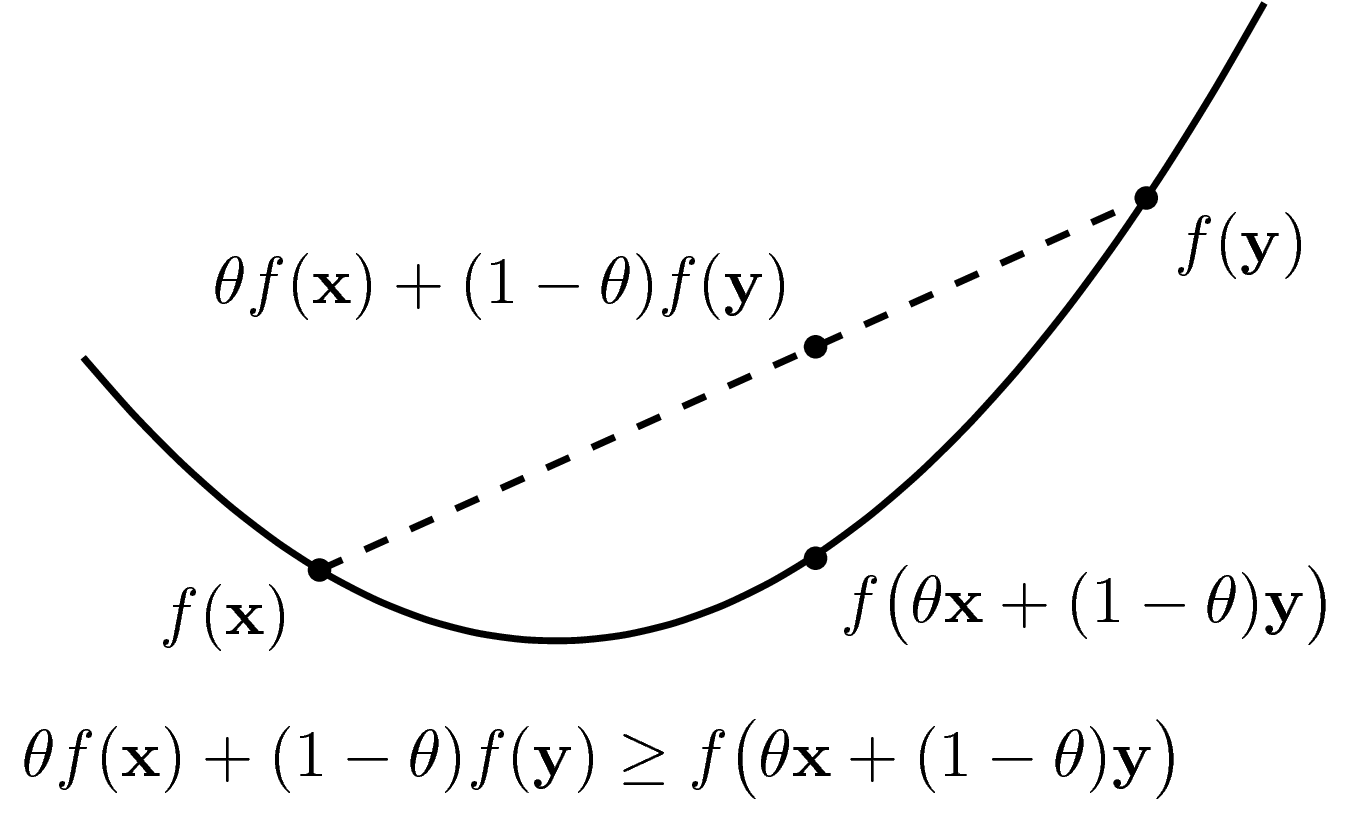
\includegraphics[width=0.6\linewidth]{Chapter2/Chapter2Figs/convexf_def}
	\caption{Hàm lồi.}
	\label{fig:hamloi}
\end{figure}

Trong khóa luận này có đề cập đến tối ưu cực đại hàm lõm. Do vậy nều $-f(x)$ là hàm lồi thì $f(x)$ là hàm lõm. Với lợi thế của bài toán có hàm mục tiêu là hàm lồi/ lõm ta luôn luôn tìm được điểm cực đại hoặc cực tiểu tốt nhất (global minimum/ maximum). Hình \ref{fig:convexnonconvex} minh họa hàm lồi và không lồi. Dễ dàng thấy được ở hàm lồi luôn chỉ có duy nhất một điểm cực tiểu ngược lại ở hàm không lồi luôn có các điểm cực tiểu địa phương và cực đại địa phương như vậy rất khó khăn hoặc bất khả thi trong việc xác định điểm cực tiểu tốt nhất cho bài toán.
\begin{figure}[H]
	\centering
	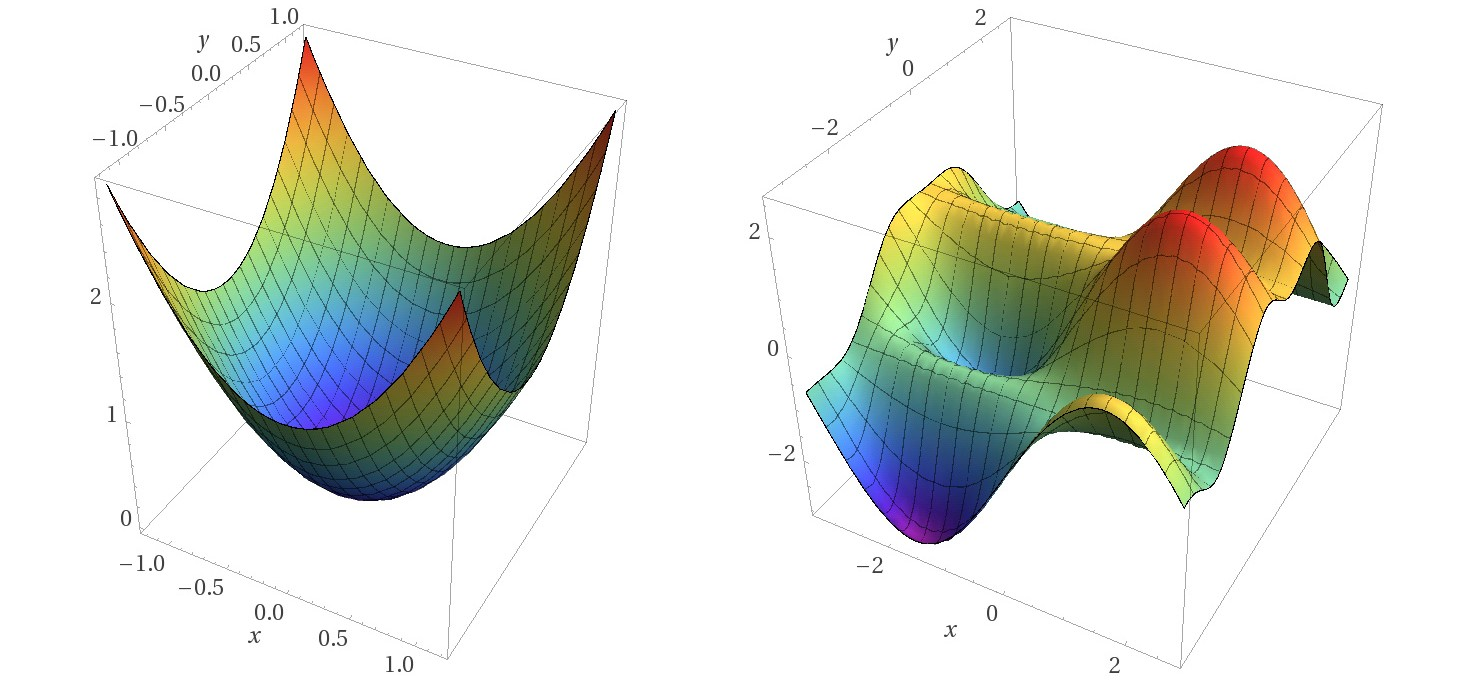
\includegraphics[width=1\linewidth]{Chapter2/Chapter2Figs/convexandnoconvex.jpg}
	\caption{Hàm lồi (trái) và hàm không lồi (phải)}
	\label{fig:convexnonconvex}
\end{figure}
\nomenclature[KN]{GD}{Gradient descent}
\nomenclature[KH]{$J(\theta)$}{Hàm chi phí}
\nomenclature[KH]{$\nabla_\theta f\left( \theta\right)$}{Đạo hàm của hàm số $f\left( \theta\right)$ theo $\theta$}
\nomenclature[KH]{$\alpha$}{Tham số tốc huấn luyện}
Một trong những phương pháp tối ưu hàm lồi được sử dụng rộng rãi cho học máy chính là phương pháp tăng\ giảm gradient nhằm ước lượng tham số $\theta$ của hô mình, khi $J(\theta)$ khả vi. Phương pháp này được trình bày trong thuật toán \ref{alg:GD} \cite{boyd2004convex} dưới đây:
\begin{algorithm}\caption{\label{alg:GD} Batch gradient descent method.}
	\begin{algorithmic}[1]
		\STATE \textbf{Given} bắt đầu từ một điểm $\theta = \{\theta_1,\dots,\theta_n\} \in \textbf{dom} f$
		\REPEAT
		\STATE 1. $\Delta \theta:=-\nabla_\theta f\left( \theta\right) $.
		\STATE 2. \text{Chọn bước nhảy $\alpha$ mặc định hoặc thông qua thuật toán backtracking line search}
		\STATE 3. \textit{Cập nhật.} $\theta:=\theta+\alpha\Delta \theta$
		\UNTIL{thuật toán hội tụ.}
	\end{algorithmic}
\end{algorithm}

Trong thuật toán \ref{alg:GD} có sử dụng phương pháp xác định $\alpha$ là tham số thể hiện bước nhảy hay tốc độ huấn luyện của thuật toán. Hình \ref{fig:learningrate} khi $\alpha$ quá lớn lớn hoặc quá nhỏ đều sẽ làm ảnh hưởng đến thời gian hội tụ của bài toán. Vì vậy trong các thuật toán giảm gradient, tốc độ học $\alpha$ cần được thay đổi phù hợp theo mỗi lần lặp. Thuật toán \ref{alg:Backtrackingls} \cite{luenberger1973introduction} được sử dụng phổ biến để xác định giá trị $\alpha$ qua mỗi lần lặp, có dễ hiểu hơn về phương pháp thông qua cách nghĩ trước nước đi trong chơi cờ.

\begin{figure}[H]
	\centering
	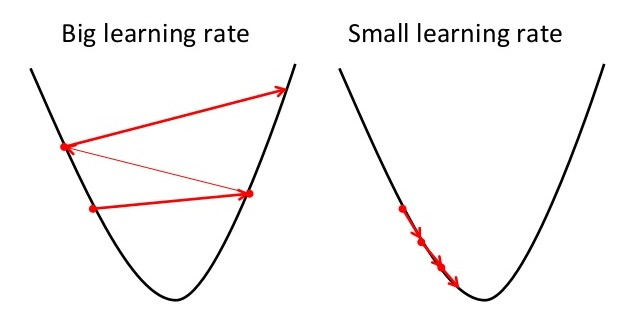
\includegraphics[width=0.8\linewidth]{Chapter2/Chapter2Figs/learningrate.jpg}
	\caption{Sự ảnh hưởng của $\alpha$ đến quá trình huấn luyện.}
	\label{fig:learningrate}
\end{figure}
\begin{algorithm}\caption{\label{alg:Backtrackingls}Backtracking line search.}
	\begin{algorithmic}
		\STATE \textbf{Given} bắt đầu tại một điểm $\bigtriangleup \theta$ với f tại $\theta \in \textbf{dom} f, \gamma \in (0,0.5), \beta \in (0,1)$
		\STATE \textbf{While} $f(\theta + \alpha\bigtriangleup \theta) > f(\theta) + \gamma\alpha\nabla f(\theta)^T \bigtriangleup \theta$ \\
		{$\alpha = \beta \alpha$}
	\end{algorithmic}
\end{algorithm}

Với hàm mục tiêu có độ phức tạp thì việc tính $\nabla f\left( x\right)$ đòi hỏi khối lượng tính toán lớn. Và nếu dữ liệu có kích thước $N$ lớn thì mỗi bước lặp có khối tượng tính toán lớn, thuật toán chạy chậm. Do vậy để tiết kiệm khối lượng tính toán, thuật toán \ref{alg:SGD} \cite{bottou2010large} phương pháp giảm gradient ngẫu nhiên là một phương pháp phù hợp trong huấn luyện dữ liệu lớn.
\nomenclature[KN]{$SGD$}{Stochastic Gradient descent}
\begin{algorithm}[H]\caption{\label{alg:SGD}Stochastic Gradient descent method.}
	\begin{algorithmic}[1]
		\STATE \textbf{Given} bắt đầu tại $\theta=\{\theta_1,\dots,\theta_n\} \in \textbf{dom} f$
		\REPEAT
		\STATE 1. Xáo trộn tập dữ liệu huấn luyện
			\FOR{ $i = 1 : N$}
				\STATE 1. $\Delta \theta:=-\nabla_\theta f\left( \theta;x^i,y^i \right) $.
				\STATE 2. \text{Chọn bước nhảy $\alpha$ mặc định hoặc thông qua thuật toán backtracking line search}
				\STATE 3. \textit{Cập nhật.} $\theta:=\theta+\alpha\Delta \theta$
			\ENDFOR
		\UNTIL{thuật toán hội tụ.}
	\end{algorithmic}
\end{algorithm}

Thuật toán \ref{alg:MBSGD} \cite{konevcny2016mini} là sự kết hợp của hai thuật toán trên phù hợp chạy trên những hệ thống tính toán song song/ phần tán được đề cập trong chương \ref{chap:c4}.
\nomenclature[KN]{$MBSGD$}{Mini-batch Stochastic Gradient descent}
\begin{algorithm}[H]\caption{\label{alg:MBSGD}Mini-batch Stochastic gradient descent method.}
	\begin{algorithmic}[1]
		\STATE \textbf{Given} bắt đầu tại $\theta=\{\theta_1,\dots,\theta_n\} \in \textbf{dom} f$ và chọn $0 \leq k \leq N$
		
		\REPEAT
		\STATE 1. xáo trộn tập dữ liệu huấn luyện
		\FOR{ $i = 1 ; i\leq N;i+=k$}
		\STATE 1. $\Delta \theta:=-\nabla_\theta f\left( \theta;x^{i:i+k},y^{i:i+k} \right) $.
		\STATE 2. \text{Chọn bước nhảy $\alpha$ mặc định hoặc thông qua thuật toán backtracking line search}
		\STATE 3. \textit{Cập nhật.} $\theta:=\theta+\alpha\Delta \theta$
		\ENDFOR
		\UNTIL{thuật toán hội tụ.}
	\end{algorithmic}
\end{algorithm}



	\chapter{Phương pháp phát hiện cộng đồng dựa trên mô hình BigCLAM}\label{chap:c3}
\ifpdf
    \graphicspath{{Chapter3/Chapter3Figs/PNG/}{Chapter3/Chapter3Figs/PDF/}{Chapter3/Chapter3Figs/}}
\else
    \graphicspath{{Chapter3/Chapter3Figs/EPS/}{Chapter3/Chapter3Figs/}}
\fi
Một trong những vấn đề của các thuật toán phát hiện cộng đồng hiện nay là khả năng xử lý các mạng lớn lên tới hàng triệu đỉnh và cạnh nối. Đặc biệt là bài toán phát hiện cộng đồng chồng chéo càng là một vấn đề. Năm 2012, đồng tác giả hai nhà khoa học Yang and Leskovec
[2012] \cite{yang2012community} đã đề giới thiệu mô hình AGM (Community-Affiliation Graph Model) cho phướng pháp phát hiện cộng đồng chồng chéo. Và một năm sau đó họ đã đề xuất phương pháp phát hiện cộng đồng lớn dựa trên mô hình AGM và đặt tên là mô hình BigCLAM (Community Affiliation Model for BigNetworks).

Trong chương này, tôi sẽ trình bày chi tiết phương pháp phát hiện cộng đồng có tính chồng chéo dựa trên mô hình BigCLAM được đề suất bởi Yang and Leskovec [2013] \cite{yang2013overlapping}. 

\section{Mô hình BigCLAM}

Trong phần này, tôi sẽ trình bày ngắn gọn mô hình cộng đồng cho đồ thị/ mạng mà BigCLAM sử dụng. Mô hình BigCLAM phần lớn vẫn dựa trên mô hình hai nhà khoa học đề xuất là AGM, một đồ thị hai phần thể hiện sự liên kết giữa các cộng đồng và các đỉnh trong mạng (hình \ref{fig:bigclam-diagram}), được ký hiệu là $B(\mathcal{V},\mathcal{C},\mathcal{M})$. Mặc dù không giống như AGM, BigCLAM không có xác suất kết nối trên mỗi cộng đồng, nhưng thay vào đó từ mỗi cộng đồng sẽ có một trọng số liên kết đến từng phần tử. Mô hình gán một trọng số không âm $F_{vc}(v \in \mathcal{V}, c \in \mathcal{C})$ trên mỗi cạnh của đồ thị phân đôi được thể hiện như là độ liên kết của quan hệ giữa một đỉnh trong mạng đến cộng đồng.
\nomenclature[KH]{$F$}{Matrix trọng số kết nối cộng đồng}
\nomenclature[KH]{$F_u$}{Vector trọng số kết nối cộng đồng}
\nomenclature[KH]{$p(u,v)$}{Xác suất tạo ra cạnh $(u,v) \in \mathcal{E}$}
\begin{definition}(Matrix và vector trọng số kết nối cộng đồng)
	
	Một matrix không âm $F =  (F_{vc})\in \mathbb{R}^{|\mathcal{V}|\times|\mathcal{C}|}$ ($F_{vc} \geq 0$) biểu diễn các trọng số liên kết giữa các đỉnh đến các cộng đồng. Một vector không âm $F_u =  (F_{uc} \geq 0)\in \mathbb{R}^{|\mathcal{V}|}$ biểu diễn các trọng số kết nối giữa đỉnh $u$ đến tất cả các cộng đồng (Hình \ref{fig:bigclam-diagram}). Với $F$, mô hình BigCLAM sinh đồ thị $G(\mathcal{V}, \mathcal{E})$ bằng tạo các cạnh $(u,v)$ với xác suất $p\left(u,v\right)$:
	\begin{equation}\label{eq:p_uv}
		p\left(u,v\right) = 1 -\exp(-F_u\cdot F_v^T) = 1 - \exp\left(-\sum_{c\in \mathcal{C}}{F_{uc}F_{vc}}\right)
	\end{equation}
\end{definition}
\begin{figure}[H]
	\centering
	\begin{minipage}[t]{0.48\textwidth}
		\centering
		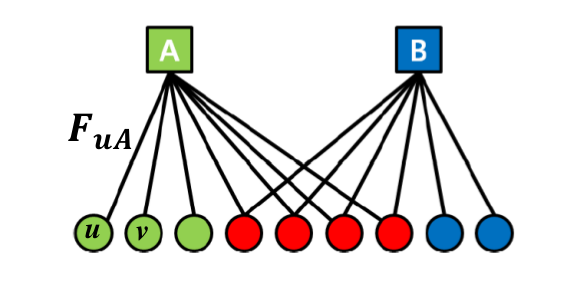
\includegraphics[width=\linewidth]{Chapter3/Chapter3Figs/bigclam-diagram}
		\caption{Mô hình cộng đồng BigCLAM}
		\label{fig:bigclam-diagram}
	\end{minipage}
	\begin{minipage}[t]{0.48\textwidth}
		\centering
		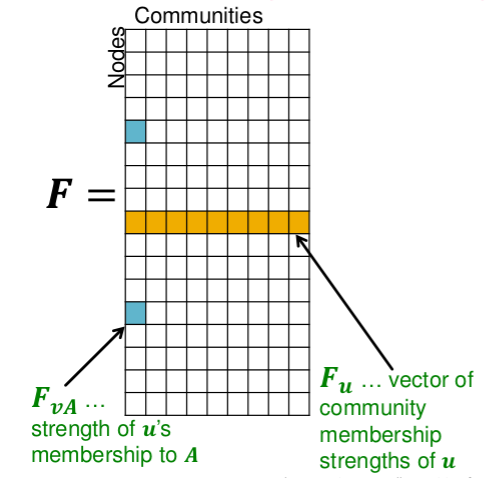
\includegraphics[width=0.7\linewidth]{Chapter3/Chapter3Figs/fmatrixvector.png}
		\caption{Matrix trọng số kết nối cộng đồng}
		\label{fig:matrixbigclam-diagram}
	\end{minipage}    
\end{figure}
Hay nói cách khác, công thức \ref{eq:p_uv} được hiểu như sau. Ta giả sử rằng mỗi cộng đồng $c \in \mathcal{C}$ kết nối đến các thành viên của nó $u,v \in \mathcal{V}$ hoàn toàn độc lập với xác suất là $1-\exp(-F_{uc}\cdot F_{vc})$ thì xác suất tạo ra cạnh $(u,v) \in \mathcal{E}$ sẽ là $1-\exp(-F_{uc}\cdot F_{vc})$. Định nghĩa này dựa trên quan sát của tác giả cho rằng với mỗi tập đỉnh là thành phần chung của sự chồng chéo các cộng đồng sẽ thu được xác suất cao hơn các tập không chồng chéo.

Công thức \ref{eq:p_uv} rõ ràng cho thấy BigCLAM tạo nên sự chồng chéo của các cộng đồng. Nó tạo ra một mối quan hệ giữa xác suất cạnh và số lượng cộng đồng chia sẻ. Điều này là do thực tế là các đỉnh chia sẻ nhiều thành viên cộng đồng nên nhận được nhiều cơ hội để tạo một cạnh trong đồ thị. Ví dụ, các cặp nút màu đỏ trong vùng chồng chéo của các cộng đồng $A$ và $B$ trong hình \ref{fig:bigclam-diagram} có hai cơ hội để tạo ra một cạnh. Đầu tiên chúng tạo ra một cạnh với xác suất $1-\exp(-F_{uA}. F_{vA})$ (do là thành viên của cộng đồng $A$) và cũng tạo ra một cạnh với xác suất $1-\exp(-F_{uB}. F_{vB})$ (do là thành viên của cộng đồng B). Như vậy xác suất cạnh giữa các đỉnh này là $1-\exp(-F_{uA}. F_{vA}  + F_{uB}. F_{vB})$. 

\section {Phát hiện cộng đồng sử dụng mô hình BigCLAM}
Với đồ thị $G(\mathcal{V},\mathcal{E})$ cho trước, mục tiêu là phát hiện ra $\mathcal{K}$ cộng đồng bằng cách tìm matrix $\hat{F} \in \mathbb{R}^{\mathcal{V}\times \mathcal{K}}$. Trong mục \ref{df:dn-likelihood} sẽ trình bày phương pháp xác định $\hat{F}$ thông qua việc tìm cực đại hàm khả dĩ (định nghĩa \ref{df:MLE}) $l(F) = \log P(G,F)$ 

\subsection {Cực đại hàm khả dĩ ma trận trọng số liên kết của đồ thị}\label{df:dn-likelihood}
	
	Cho $G(\mathcal{V},\mathcal{E})$ là một đồ thị với tập cạnh $\mathcal{E}$ và tập đỉnh $\mathcal{V}$, với $F=(F_{vc})\in \mathbb{R}^{|\mathcal{V}|\times|\mathcal{K}|} (v \in \mathcal{V}, c \in \mathcal{C})$ là một matrix trọng số liên kết (ở đây $\mathcal{K}$ là số cộng đồng).
	
Với mô hình trên, ta có thể thấy rằng xác suất để một tạo một cạnh $(u,v)$ trong đồ thị là $p(u,v)$ và ngược lại là $1-p(u,v)$ hay có thể viết lại như sau:
\begin{eqnarray}
	p((u,v) \in \mathcal{E}|F) = p(u,v)\\
	p((u,v) \notin \mathcal{E}|F) = 1-p(u,v)
\end{eqnarray}

Xét toàn bộ đồ thị $G(\mathcal{V},\mathcal{E})$ ta có được $P(G|F)$ chính là khả dĩ của $F$ sinh ra đồ thị $G$ như sau:
\begin{equation}
\begin{array}{lll}
	\mathcal{L}(F|G) = P(G|F)
	&= \prod_{(u,v) \in \mathcal{E}}{p(u,v)}\prod_{(u,v) \neq \mathcal{E}}{(1-p(u,v))}\\
	&= \prod_{(u,v) \in E}{(1 - \exp(-F_uF_v^T))}\prod_{(u,v) \neq \mathcal{E}}{\exp(-F_uF_v^T)}.
\end{array}
\end{equation}
Đây là một dang bài toán ước lượng tham số bằng cực đại hàm khả dĩ (Maximum likelihood estimation). Theo định nghĩa \ref{df:MLE} ta được hàm log-likelihood $l(F)$ sau:
\begin{equation}\label{ct:loglikelihood}
	l(F) = log \mathcal{L}(F|G) = \sum_{(u,v) \in \mathcal{E}}{(log(1-\exp(-F_uF_v^T)) - \sum_{(u,v)\neq \mathcal{E}}{\exp(F_uF_v^T})}.
\end{equation}
Mặt khác hàm logarit là đơn điệu tăng nên $\hat{F}$ cực đại $l(F)$ thì cũng là cực đại log $P(G|F)$ tức là:

\begin{equation} \label{eq:ctf_hat}
	\hat{F} = \arg \max_{F \geq 0} \mathcal{L}(F) = \arg \max_{F \geq 0} l(F) 
\end{equation}

Từ công thức \ref{ct:loglikelihood}, ta giả sử với $\mathcal{K}$ cộng đồng đã biết (phương pháp tìm $\mathcal{K}$ sẽ được đề cập ở phần sau) ta cần giải quyết bài toán trong công thức \ref{eq:ctf_hat}. Nhưng thay vì phải cực đại $l(F)$ ta sẽ tách thành các bài toán tìm cực đại $l(F_u)$ và cập nhật lại $F_u$ trên từng đỉnh $u \in \mathcal{V}$ theo các $F_v,v\neq u$ như sau:

\begin{equation}\label{eq:ctfu_hat}
\hat{F_u} = \arg \max_{F_{uc}, c \in \mathcal{C}} l(F_u) 
\end{equation}
Trong đó: 
\begin{equation}\label{eq:ctfu_l}
l(F_u) = \sum_{v \in \mathcal{N}(u)}{log(1 - \exp(-F_u F_v^T))} - \sum_{v \notin \mathcal{N}(u)}{F_uF_v^T}
\end{equation}
$\mathcal{N}(u)$ là tập các đỉnh lân cận của $u$ (Định nghĩa \ref{df:dinhlancan})

Ta thấy rằng $l(F_u)$ là một hàm lõm như vậy vấn đề trên được coi như là bài toán tối ưu hàm lõm và có thể tìm được điểm cực đại duy nhất một cách dễ dàng. Để ước lượng được các vector $F_u$ (công thức \ref{eq:ctfu_hat}) ta sử dụng các phương pháp tối ưu hàm lồi/ lõm được trình bày ở mục \ref{muc:toiuuhamloi}
\begin{equation}\label{eq:gradian}
l'(F_u) = l(F_u)+\alpha \bigtriangledown(l(F_u))
\end{equation}
Trong đó građian cho log-likelihood của $F_u$ là:
\begin{equation}\label{eq:ctfu_l1}
\bigtriangledown(l(F_u))=\dfrac{\partial l(F_u)}{\partial F_u} = \sum_{v \in \mathcal{N}(u)}{F_v \dfrac{\exp(-F_u F_v^T)}{1-\exp(-F_u F_v^T)}} - \sum_{v \notin \mathcal{N}(u)}{F_v}
\end{equation}

Để giảm độ phức tạp tính toán xuống còn $O(|\mathcal{N}(u)|)$ tôi xin biến đổi lần lượt các công thức \ref{eq:ctfu_l} \ref{eq:ctfu_l1} như sau:

\begin{equation}\label{eq:caitien}
\sum_{v \notin \mathcal{N}(u)} {F_u F_v^T}= \sum_{v} {F_u F_v^T} - \sum_{v \in N(u)} {F_u F_v^T}
\end{equation}

\begin{equation}\label{eq:caitien1}
\sum_{v \notin \mathcal{N}(u)} {F_v}= \left(\sum_{v} {F_v}\right) - F_u - \left(\sum_{v \in \mathcal{N}(u)} {F_v}\right)
\end{equation}

Matrix $F$ được cập nhật sau mỗi vòng lặp theo công thức \ref{eq:gradian}. Ta nên cho thuật toán hội tụ khi:
 \begin{equation}
 \dfrac{l'{(F_u)} - l(F_u)}{l(F_u)} < 0.0001, \forall u \in \mathcal{V}
 \end{equation}

\subsection{Khởi tạo tạo ma trận trọng số liên kết cộng đồng}
Kết quả của bài toán phát hiện cộng đồng ảnh hưởng rất nhiều từ việc khởi tạo giá tri $F_u, u\in \mathcal{V}$ cho quá trình tối ưu hàm lồi/ lõm. Để khởi tạo matrix $F$ (Định nghĩa \ref{dn:initF}), ta chọn sử dụng phương pháp tìm vùng lân cận địa phương nhỏ nhất của Gleich and Seshadhri [2011] \cite{DBLP:journals/corr/abs-1112-0031} đã được đề cập đến trong định nghĩa \ref{df:dodan} và định nghĩa \ref{df:dinhlancan}

\begin{definition}(Khởi tạo matrix trọng số liên kết)\label{dn:initF}
	
	Gọi $F$ là một matrix trọng số liên kết. $F$ được khởi tạo như sau:
	\begin{equation}
		F_{(u^{\prime})(N(u))} =
			\begin{cases}
			1 & \textit{Nếu $u^{\prime} \in N(u)$ và $N(u)$ là vùng lân cận địa phương nhỏ nhất của $u$} \\
			0 & \textit{Trường hợp còn lại}
			\end{cases}
	\end{equation}
\end{definition}
\subsection{Xác định các liên kết cộng đồng}

Sau khi công thức \ref{eq:ctf_hat} hội tụ, ta sẽ có được một matrix trọng số liên kết $F$. Tuy nhiên ta cần phải xác định đỉnh $u$ có thuộc cộng đồng $c$ hay không. Vì vậy ta phải lựa chọn một ngưỡng $\delta$ cho matrix $F$ qua định nghĩa \ref{dn:xacdinhlienketcd}.
\begin{definition}(Xác định liên kết cộng đồng) \label{dn:xacdinhlienketcd}
	Cho $G(\mathcal{V},\mathcal{E})$, $F$ là matrix trọng số liên kết của $G$ và $\epsilon = \dfrac{2|E|}{|V|(|V| - 1)}$.
	
	Thuật toán xét $u \in \mathcal{V}$ như một thành viên trong cộng đồng $c\in \mathcal{C}$ nếu thỏa mãn $F_{uc}\geq \delta = \sqrt{-\log(1-\epsilon)}$.
\end{definition}

\subsection{Xác định số cộng đồng}
Trong phần đầu của chương này đã tiền hành xây dựng mô hình với giả sử $\mathcal{K}$ số cộng đồng trong $G(\mathcal{V},\mathcal{E})$ đã biết. Yang và Leskovec đã trình bày một phương pháp để ước lượng gần nhất số cộng đồng $\mathcal{K}$ vẫn dựa trên phương pháp cực đại hàm khả dĩ như sau:
\begin{itemize}
	\item Chọn ngẫu nhiên $20\%$ cặp đỉnh cho $H$;
	\item Với mỗi $\mathcal{K}$ là số cộng đồng. $\mathcal{K} \in [minCom;maxCom]$ với bước nhảy trong khoảng $[minCom; maxCom]$ là $\alpha = \exp{\left(\log{\left(\dfrac{maxCom}{minCom}\right)}\times\dfrac{1}{divCom}\right)}$. Trong đó $minCom$ là số cộng đồng nhỏ nhất, $maxCom$ là số cộng đồng lớn nhất và $divCom$ là số lượng $\mathcal{K}$ muốn thử.
	\begin{itemize}
			\item Chạy thuật toán phát hiện cộng đồng, với $\mathcal{K}$ là số cộng đồng mong muốn pháy hiện
			\item Đánh giá likelihood của matrix trọng số trên tập $H$, $l_k{(F_H)}$.
		\end{itemize}
	\item $\hat{\mathcal{K}} = \arg \max_K l_k{(F_H)}$.
\end{itemize} 

\section{Đánh giá hiệu năng}
Theo kết quả của các tác giả khi so sánh hiệu năng  giữa giữa BigCLAM và các mô hình được sử dụng để phát hiện cộng đồng như LC \cite{ahn2010link}, CPM \cite{palla2005uncovering}, MMS \cite{airoldi2008mixed}. Hình \ref{fig:bigclamcomparis} cho thấy BigCLAM cho hiệu năng cao hơn từ $10$ đến $100$ lần so với phương pháp còn lại. 

\begin{figure}[H]
	\centering
	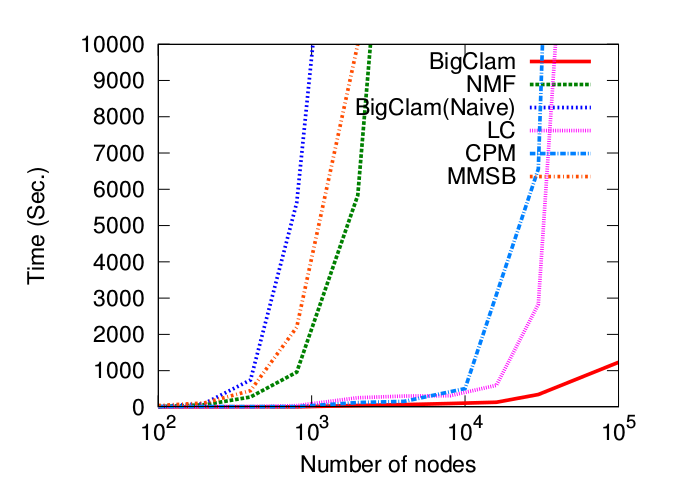
\includegraphics[width=0.6\linewidth]{Chapter3/Chapter3Figs/bigclamcomparis}
	\caption{So sánh hiệu năng của các mô hình với BigCLAM}
	\label{fig:bigclamcomparis}
\end{figure}

Ngoài ra các tác giả sử dụng một số mạng đã được xác định trước các cộng đồng (ground-truth communities) để đánh giá độ chính xác của các mô hình được dùng để phát hiện cộng đồng. Bảng \ref{comtruth} dưới đây là thông tin các mạng được sử dụng.

\begin{table}[H]
	\centering
	\caption{Mô tả các mạng sử dụng để thực nghiệm}
	\label{comtruth}
	\begin{tabular}{@{}lrrr@{}}
		\toprule
		Tên mạng                & Số đỉnh      & Số cạnh         & Số cộng đồng \\ \midrule
		Mạng xã hội LiveJournal & $3,997,962$  & $34,681,189$    & $287,512$    \\
		Mạng xã hội Friendster  & $65,608,366$ & $1,806,067,135$ & $957,154$    \\
		Mạng xã hội Ourkut      & $3,072,441$  & $117,185,083$   & $6,288,363$  \\
		Mạng xã hội Youtube     & $1,134,890$  & $2,987,624$     & $8,385$      \\
		Mạng cộng tác DBLP      & $317,080$    & $1,049,866$     & $13,477$     \\
		Mạng bán hàng Amazon    & $334,863$    & $925,872$       & $75,149$     \\ \bottomrule
	\end{tabular}
\end{table}
Tác giả sử dụng các thang đo đánh giá như sau:
\begin{itemize}
	\item \textbf{Average $F1$ score} \citep{1742-5468-2011-02-P02017} : Thể hiện mức độ chính xác trung bình của các cộng đồng phát hiện được với các cộng đồng thực tế.
	\item \textbf{Omega Index} \cite{gregory2011fuzzy}: Là chỉ số thể hiện độ chính xác số cộng đồng mà mỗi đỉnh thuộc.
	\item \textbf{Accuracy in the number of communities}:Độ chính xác về số lượng cộng đồng
\end{itemize}
Hình \ref{fig:ground-truthcommunities} là kết quả của sự so sánh hiệu năng giữa các mô hình trên một số mạng. Dễ dàng thấy được, hiệu năng trung bình của mô hình BigCLAM là $3.60$ cao hơn hơn các mô hình còn lại như Link Clustering ($2.01$), CPM ($2.47$) và MMSB ($3.14$). Nhìn chung, BigCLAM có hiệu năng tương đối tốt, tỏ ra khá vượt trội so với các phương pháp thường được sử dụng và nó có khả năng phát hiện đa dạng các loại cộng đồng (chồng chéo, không chồng chéo, lồng nhau).
\begin{figure}[H]
	\centering
	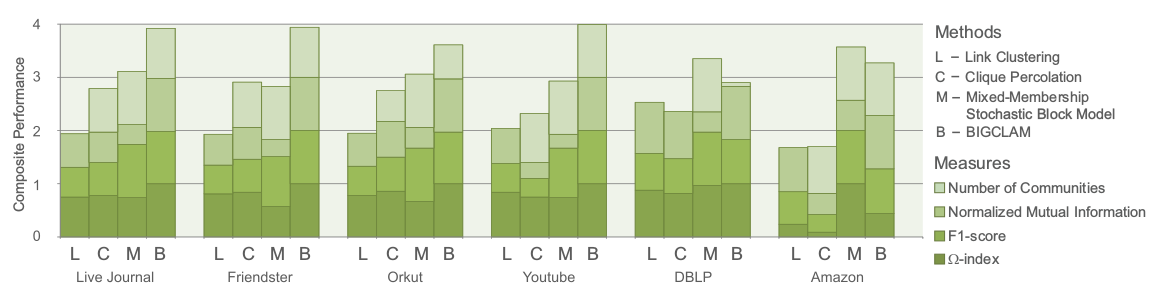
\includegraphics[width=\linewidth]{Chapter3/Chapter3Figs/ground-truthcommunities.png}
	\caption{Biểu đồ so sánh độ chính xác các mô hình trên các mạng biết trước cộng đồng}
	\label{fig:ground-truthcommunities}
\end{figure}

Mô hình BigCLAM dựa trên kỹ thuật NMF, vậy nên hoàn toàn có thể tăng tốc độ trên các kỹ thuật xử lý song song và phân tán. Trong chương \ref{chap:c4} giới thiệu và đề xuất phương pháp tăng tốc bài toán dựa trên sức mạnh xử lý trên cụm máy tính.

	\chapter{Cài đặt phương pháp phát hiện cộng đồng sử dụng mô hình BigCLAM trên hệ thống phân tán}\label{chap:c4}
\ifpdf
    \graphicspath{{Chapter3/Chapter3Figs/PNG/}{Chapter3/Chapter3Figs/PDF/}{Chapter3/Chapter3Figs/}}
\else
    \graphicspath{{Chapter3/Chapter3Figs/EPS/}{Chapter3/Chapter3Figs/}}
\fi
Chương này sẽ trình bày ngắn gọn về hệ thống tính toán và lưu trữ phân tán sử dụng Apache Spark/ Hadoop framework trong xử lý dữ liệu lớn. Cuối cùng, tôi sẽ trình bày quá trình cài đặt phương pháp phát hiện cộng đồng dựa trên mô hình BigCLAM trên Spark/ Hadoop.
\section{Tổng quan hệ tính toán phân tán}
\subsection{Giới thiệu Apache Hadoop \& Spark}
\nomenclature[KN]{GFS}{Google File System}
\nomenclature[KN]{HDFS}{Hadoop Distributed File System}

Apache Hadoop \footnote{http://hadoop.apache.org/}, công nghệ được viết bởi Doug Cutting dựa trên hai bài báo GFS (Google File System) và MapReduce của Google vào năm 2005. Tháng Tư năm 2008, Hadoop trở thành hệ thống nhanh nhất để sắp xếp (sort) 1 terabyte dữ liệu, khi mất 209 giây chạy trên cluster gồm 910 nodes, đánh bại kỷ lục cũ là 297 giây. Tháng 11 năm 2008, Google thông báo hệ thống MapReduce của họ chỉ cần 68 giây để sắp xếp 1 terabyte dữ liệu. Đến tháng 5 năm 2009, Yahoo sử dụng Hadoop chỉ cần 62 giây để làm việc tương tự. Từ đó đến nay, cả một hệ sinh thái đã được xây dựng lấy Hadoop làm nòng cốt để giải quyết những bài toán về dữ liệu lớn.


Hadoop bao gồm hai thành phần chính (Hình \ref{fig:hadoop}):
\begin{itemize}
	\item \textbf{HDFS:} Hadoop Distributed File System, hệ thống tập tin phân tán, cho phép lưu trữ dữ liệu trên cluster gồm nhiều máy tính có cấu hình ở mức thông thường
	\item \textbf{MapReduce framwork}: cho phép xử lý dữ liệu song song trên cluster.
\end{itemize}

Trên nền tảng hai thành phần đó, cộng đồng mã nguồn mở đã phát triển thêm rất nhiều công cụ khác giúp tăng hiệu quả khi làm việc với Hadoop (Hình \ref{fig:hadoop}):
\begin{itemize}
\item Hbase: Cơ sở dữ liệu NoSQL, được xây dựng trên nền của HDFS, hỗ trợ những dữ liệu phi cấu trúc.

\item Flume: Dùng để thu thập dữ liệu từ các nguồn như log hệ thống

\item Oozie: Định nghĩ mối tương quan giữa các tác vụ và lập luồng làm việc cho MapReduce.

\item Hive: Sử dụng những câu lệnh như SQL và biên dịch những câu lệnh này thành tập hợp các tác vụ MapReduce.

\item Mahout: Sử dụng cho các bài toán về học máy.

\item Sqoop: Dùng để chuyển đổi dữ liệu từ các cơ sở dữ liệu quan hệ sang HDFS.
\end{itemize}

\begin{figure}[H]
	\centering
	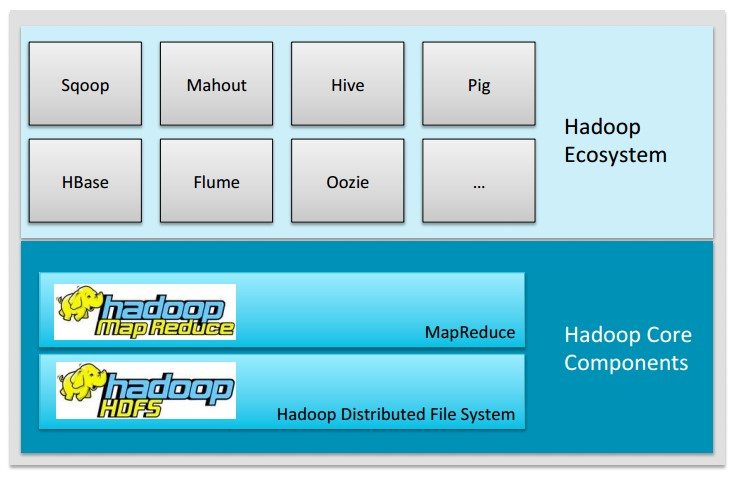
\includegraphics[width=0.9\linewidth]{Chapter4/Chapter4Figs/hadoop}
	\caption{Kiến trúc và hệ sinh thái của Apache Hadoop}
	\label{fig:hadoop}
\end{figure}

Matei Zaharia, cha đẻ của Spark, sử dụng Hadoop từ những ngày đầu. Đến năm $2009$ ông viết Apache Spark\footnote{http://spark.apache.org/} để giải quyết những bài toán học máy ở đại học UC Berkely vì Hadoop MapReduce hoạt động không hiệu quả cho những bài toán này. Rất sớm sau đó ông nhận ra rằng Spark không chỉ hữu ích cho học máy mà còn cho cả việc xử lý luồng dữ liệu hoàn chỉnh. Spark cho phép thực hiện tính toán cùng lúc trên toàn bộ tập dữ liệu mà không cần phải trích xuất mẫu tính toán thử nghiệm. Tốc độ xử lý của Spark có được do việc tính toán được thực hiện cùng lúc trên nhiều máy khác nhau. Đồng thời việc tính toán được thực hiện ở bộ nhớ trong (in-memories) hay thực hiện hoàn toàn trên RAM.

Khi ta có một tác vụ nào đó qúa lớn mà không thể xử lý trên một máy tính/ server, Spark cho phép ta phân chia tác vụ này thành những phần dễ quản lý hơn. Sau đó, Spark sẽ chạy các tác vụ này trong bộ nhớ trên các cluster của nhiều máy tính/server khác nhau để khai thác tốc độ truy xuất nhanh từ RAM. Spark sử dụng API Resilient Distributed Dataset (RDD) để xử lý dữ liệu. Spark nhanh hơn khá nhiều so với cách tiếp cận MapReduce truyền thống.Theo như giới thiệu từ trang chủ của Apache Spark, thì tốc độ của nó nhanh hơn $100x$ so với Hadoop MapReduce khi chạy trên bộ nhớ, và nhanh hơn $10x$ lần khi chạy trên đĩa, tương thích hầu hết các CSDL phân tán (HDFS, HBase, Cassandra, ...). Ta có thể sử dụng Java, Scala, Python hoặc R để triển khai các ứng dụng trên Spark.
\begin{figure}[H]
	\centering
	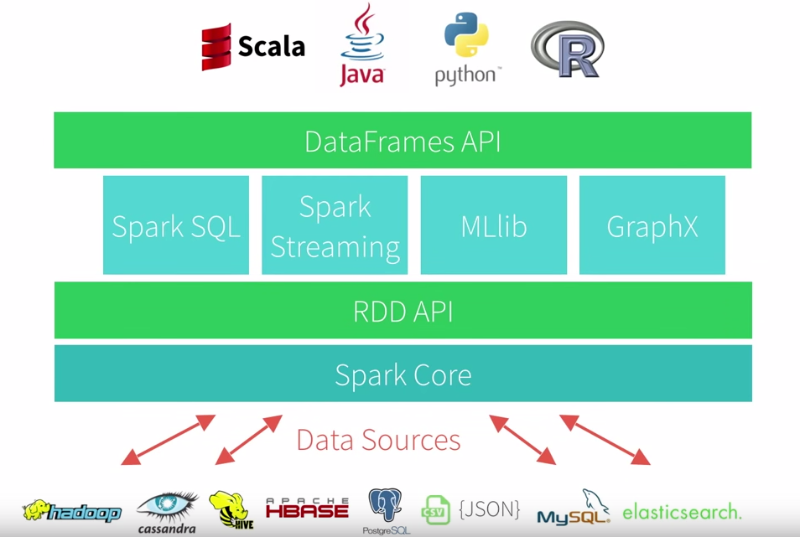
\includegraphics[width=0.9\linewidth]{Chapter4/Chapter4Figs/sparkecosystems}
	\caption{Kiến trúc và hệ sinh thái Apache Spark}
	\label{fig:spark}
\end{figure}

Kiến trúc và hệ sinh thái của Apache gồm:
\begin{itemize}
	\item \textbf{Spark Core:} cung cấp những chức năng cơ bản nhất của Spark như lập lịch cho các tác vụ, quản lý bộ nhớ, fault recovery, tương tác với các hệ thống lưu trữ\dots Đặc biệt, Spark Core cung cấp API để định nghĩa RDD (Resilient Distributed DataSet) là tập hợp của các item được phân tán trên các node của cluster và có thể được xử lý song song.
	\item \textbf{Spark SQL} cho phép truy vấn dữ liệu cấu trúc qua các câu lệnh SQL. Spark SQL có thể thao tác với nhiều nguồn dữ liệu như Hive tables, Parquet, và JSON;
	\item \textbf{Spark Streaming} cung cấp API để dễ dàng xử lý dữ liệu stream;
	\item \textbf{MLlib} Cung cấp rất nhiều thuật toán của học máy như: classification, regression, clustering, collaborative filtering\dots
	\item \textbf{GraphX} là thư viện để xử lý đồ thị.
\end{itemize}
Spark có thể chạy trên nhiều loại Cluster Managers như Hadoop YARN, Apache Mesos hoặc trên chính cluster manager được cung cấp bởi Spark được gọi là Standalone Scheduler.

Một trong những lý do khiến Spark chạy nhanh hơn Hadoop MapReduce đó là ở mỗi tác vụ dữ liệu được nạp lên bộ nhớ và xử lý ở đó, những tác vụ sau có thể sử dụng dữ liệu nằm trên bộ nhớ thay vì phải đọc ghi liên tục vào HDFS như Hadoop MapReduce. Theo một so sánh, năm $2013$ Hadoop sử dụng cluster bao gồm $2100$ máy và mất $72$ phút để sắp xếp $100 TB$ dữ liệu, trong khi Spark cần số lượng máy bằng $1/10$ nhưng sắp xếp chỉ mất $23$ phút. Trong nhiều trường hợp Spark có thể chạy nhanh hơn từ $30-50$ lần so với Hadoop MapReduce.

\begin{figure}[H]
	\centering
	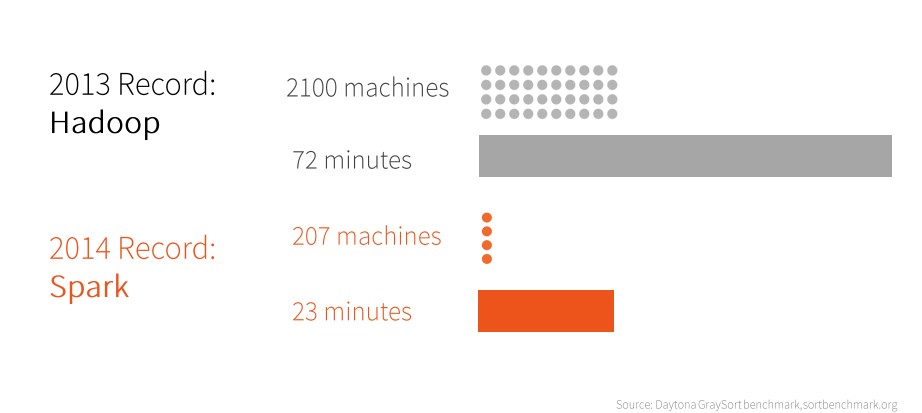
\includegraphics[width=0.9\linewidth]{Chapter4/Chapter4Figs/stark5}
	\caption{So sánh tốc độ sắp xếp $1TB$ dữ liệu của Apache Hadoop và Apache Spark}
	\label{fig:stark5}
\end{figure}

Năm $2015$, Spark trở thành dự án mã nguồn mở sôi động nhất trong lĩnh vực dữ liệu lớn khi thường xuyên được cập nhật bởi hơn $800$ lập trình viên từ $200$ công ty trên khắp thế giới.
\begin{figure}[H]
	\centering
	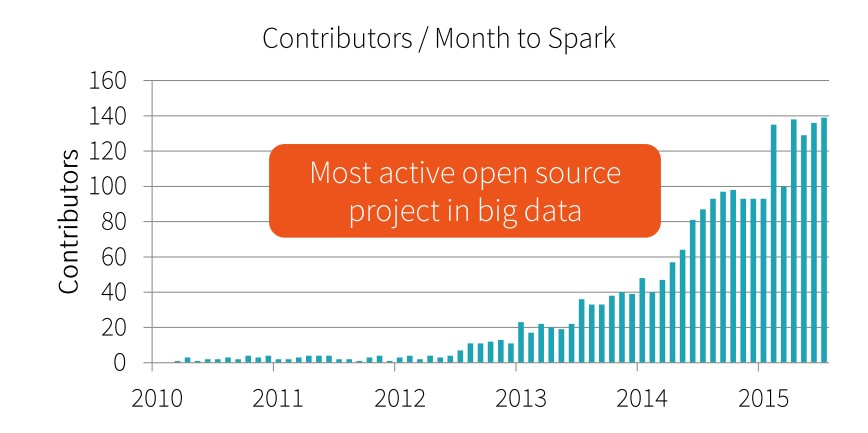
\includegraphics[width=0.9\linewidth]{Chapter4/Chapter4Figs/stark8}
	\caption{Biểu đồ thể hiện sự quan tâm của cộng đồng đến Apache Spark}
	\label{fig:stark8}
\end{figure}


Hình \ref{fig:databricks_2016_spark_survey1} cho thấy các ngôn ngữ và hệ sinh thái của spark được sử dụng trong lập trình các ứng dụng. Dễ thấy Scala và Python là hai ngôn ngữ được sử dụng nhiều nhất trên $58\%$. Các thành phần trong hệ sinh thái được sử dụng khá đồng đều, được sử dụng nhiều nhất là Dataframes và Spark SQL.
\begin{figure}[H]
	\centering
	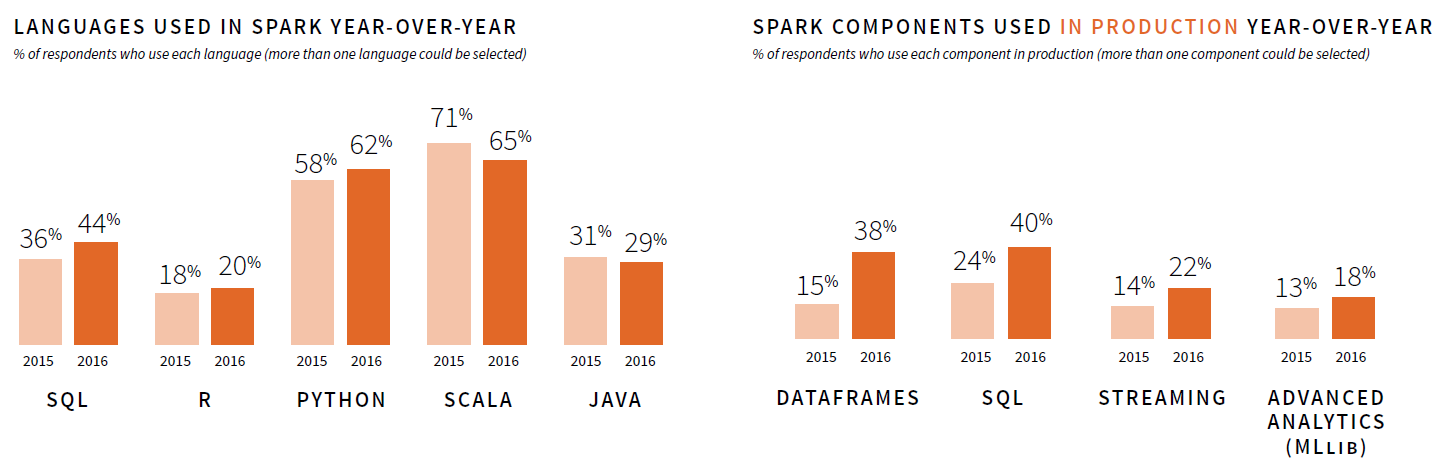
\includegraphics[width=\linewidth]{Chapter4/Chapter4Figs/databricks_2016_spark_survey1.PNG}
	\caption{Biểu đồ thể hiện sự so sánh mức độ quan tâm của các hệ sinh thái Apache Spark}
	\label{fig:databricks_2016_spark_survey1}
\end{figure}

Trong phần phụ lục A đã trình bày chi tiết cách cài đặt và bảng danh sách các lệnh cơ bản khi làm việc trên hai Apache Hadoop \& Spark.

Đề tài này sử dụng hệ sinh thái Apache Spark cho bài toán phát hiện cộng đồng trong mạng có kích thước lớn được lưu trữ phân tán trên HDFS của Hadoop như hình \ref{fig:forrester_spark}. Cụ thể hơn bài toán sử dụng ngôn ngữ Scala do Apache Spark được xây dựng chủ yếu trên Scala vậy nên có tốc độ và hỗ trợ tốt nhất. Ngoài ra do là bài toán xử lý đồ thị lớn nên Graphx là một lựa chọn tốt.
\begin{figure}[H]
	\centering
	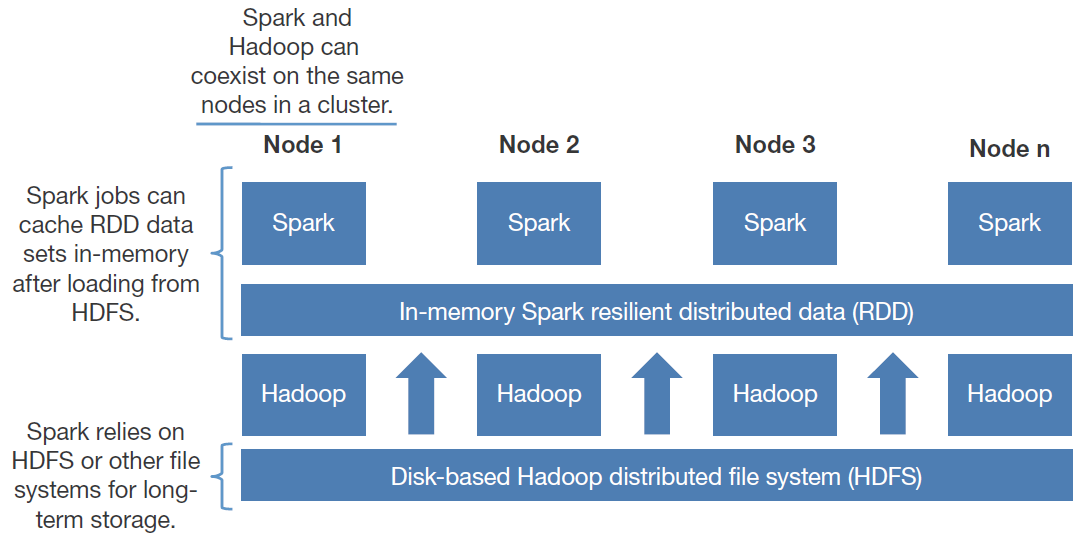
\includegraphics[width=\linewidth]{Chapter4/Chapter4Figs/forrester_spark.PNG}
	\caption{Mô hình kết hợp }
	\label{fig:forrester_spark}
\end{figure}
\subsection{Tính toán song song và phân tán với RDD}
RDD là từ viết tắt của Resilient Distributed Datasets là một cấu trúc dữ liệu cơ bản của Spark. RDD là một tập hợp bất biến phân tán của một đối tượng. Mỗi dataset trong RDD được chia ra thành nhiều phân vùng logical. Có thể được tính toán trên các node khác nhau của một cụm máy tính (cluster). RDDs API hỗ trợ các ngôn ngữ lập trình như Python, Java, Scala, R trong quá trình phát triển ứng dụng. 

Thông thường, RDD chỉ cho phép đọc, phân mục tập hợp của các bản ghi. RDDs có thể được tạo ra trong quá trình xử lý dữ liệu phân tán, RDD là một tập hợp có khả năng chịu lỗi mỗi thành phần có thể được tính toán song song.

Về cơ bản RDD hỗ trợ hai kiểu thao tác thao tác chính:
\begin{itemize}
	\item \textbf{Transformation}: Qua một phương thức transformations thì sẽ cho phép tạo mới một RDD từ RDD đã tồn tại.	Tất cả các transformation đều là lazy, có nghĩa là các transformation này sẽ không thực hiện tính toán ngay mà chúng sẽ được lưu lại thành thành các tập lệnh chờ. Quá trình này có thể hiểu như quá trình lập kết hoạch cho một công việc. Nhờ thiết kế này mà Spark chạy hiệu quả hơn.
	\item \textbf{Action}: Sẽ thực hiện lần lượt các thao tác transformations liên quan đến hành động action đã được lên lịch trước và trả về một và một tập giá trị cho chương trình điều khiển.
\end{itemize}

Bảng \ref{transformation} và \ref{action} giới thiệu các thao tác cơ bản thường được sử dụng trong quá lập trình phân tán song song.
\begin{table}[H]
	\centering
	\caption{Danh sách các thao tác transformation}
	\label{transformation}
	\begin{tabular}{p{1cm}p{5cm}p{10cm}}
		\toprule
		\textbf{STT} & \multicolumn{1}{c}{Thao tác}                        & \multicolumn{1}{c}{\textbf{Ý nghĩa}}                                                                                                                                                                                                       \\ \midrule
		1            & \textbf{map(func)}                                  & Trả về 1 RDD mới bằng cách truyền mỗi phần tử đầu vào qua hàm func.                                                                                                                                                                        \\ \midrule
		2            & \textbf{filter(func)}                               & Trả về 1 RDD mới bằng cách chọn những phần tử đầu vào(nguồn) mà hàm func,trả về kết quả true.                                                                                                                                              \\ \midrule
		3            & \textbf{flatMap(func)}                              & Tương tự map nhưng khác map ở chỗ, mỗi phần tử đầu vào quaflatMap sẽ trả về 0 hoặc nhiều phần tử đầu ra(có thể hiểu quamap sẽ là 1-1).                                                                                                     \\ \midrule
		4            & \textbf{mapPartitions(func)}                        & Tương tự như map,nhưng chạy riêng biệt trên mỗi vùng RDD,Hàmfunc, phải có dạng Iterator{[}T{]} =\textgreater  terator{[}U{]} khi chạy RDD kiểuT.                                                                                           \\ \midrule
		5            & \textbf{union(otherDataset)}                        & Trả về 1 RDD mới là hợp của tập dữ liệu phần tử đầu vào(nguồn) và các phần tử của đối(otherDataset).                                                                                                                                       \\ \midrule
		6            & \textbf{distinct({[}numTasks{]}))}                  & Trả về 1 RDD mới chứa mỗi phần tử là duy nhất của tập dữ liệunguồn.                                                                                                                                                                        \\ \midrule
		7            & \textbf{groupByKey({[}numTasks{]})}                 & Khi gọi đến 1 tập dữ liệu (K,V) sẽ trả về 1 tập là cặp (K,Seq(V))( Tức là nhóm tập các phần tử cùng Key). Chú ý: mặc định chỉ có 8 task song song khi grouping. Có thể thay đổi số task song song này bằng việc truyềnvào tham số đầu vào. \\ \midrule
		8            & \textbf{reduceByKey(func, {[}numTasks{]})}          & Khi gọi tập dữ liệu (K,V), trả về 1 tập (K,V) mà giá trị của key đượctổng hợp sử dụng hàm reduce func.                                                                                                                                     \\ \midrule
		9            & \textbf{sortByKey({[}ascending{]}, {[}numTasks{]})} & Khi gọi tập dữ liệu (K,V) với K có thể thực hiện sắp thứ tự được.Khi đó, nó sẽ trả về tập dữ liệu (K,V) được sắp sếp tăng dần hoặcgiảm dần theo key. Chú ý: ascending là kiểu Boolean.                                                     \\ \midrule
		10           & \textbf{join(otherDataset, {[}numTasks{]})}         & Khi gọi tập dữ liệu có kiểu (K,V) và (K,W), nó sẽ trả về 1 cặp mới(K,(V,W)) ( nối 2 phần tử có cùng key).                                                                                                                                  \\ \midrule
		11           & \textbf{cogroup(otherDataset, {[}numTasks{]})}      & Khi gọi tập dữ liệu có kiểu (K,V) và (K,W), nó sẽ trả về 1 tập dữ liệu (K,seq(V),seq(W)).                                                                                                                                                  \\ \midrule
		12           & \textbf{cartesian(otherDataset)}                    & Khi gọi 1 tập dữ liệu kiểu T và U, nó sẽ trả về tập dữ liệu mới (T,U).                                                                                                                                                                     \\ \bottomrule
	\end{tabular}
\end{table}

\begin{table}[H]
	\centering
	\caption{Danh sách các thao tác action}
	\label{action}
	\begin{tabular}{p{1cm}p{5cm}p{10cm}}
		\toprule
		\textbf{STT} & \multicolumn{1}{c}{Thao tác}  & \multicolumn{1}{c}{\textbf{Ý nghĩa}}                                                                                                                   \\ \midrule
		1            & \textbf{reduce(func)}         & Tổng hợp các phần tử của tập dữ liệu sử dụng hàm func(có 2 đối vàtrả về 1 kết quả).                                                                    \\ \midrule
		2            & \textbf{collect()}            & Trả về tất cả các phần tử của tập dữ liệu như 1 mảng ở driverProgram. Hàm này hữu ích sau khi lọc hoặc thao tác khác màtrả về tập dữ liệu con đủ nhỏ.  \\ \midrule
		3            & \textbf{count()}              & Trả về số phần tử của tập dữ liệu                                                                                                                      \\ \midrule
		4            & \textbf{first()}              & Trả về phần tử đầu tiên của tập dữ liệu( tương tự take(1)).                                                                                            \\ \midrule
		5            & \textbf{take(n)}              & Trả về mảng gồm n phần tử đầu tiên của tập dữ liệu.                                                                                                    \\ \midrule
		6            & \textbf{saveAsTextFile(path)} & Ghi các phần tử của tập dữ liệu như 1 file text( hoặc tập file text)lên 1 thư mục trong hệ thống local, HDFS hoặc hệ thống hỗ trợ Hadoop bất kỳ.       \\ \midrule
		7            & \textbf{countByKey()}         & Chỉ cho RDD có kiểu (K,V). Trả về 1 Map (K,Int). Int là chỉ số key.                                                                                    \\ \midrule
		8            & \textbf{foreach(func)}        & Chạy hàm func cho mỗi phần tử của tập dữ liệu. Điều này có tác dụngkhi thực hiện cập nhật 1 biến accumulator hoặc tương tác vớihệ thống lưu trữ ngoài. \\ \bottomrule
	\end{tabular}
\end{table}
%\subsection{GraphX}
%GraphX là một phần trong hệ sinh thái của Apache Spark hay có thể nói là một thư viện hỗ trợ tổ chức dữ liệu đồ thị dưới dạng phân tán trên nhiều máy trong cụm và các thuật toán hỗ trợ xử lý đồ thị. Nhờ vậy GraphX rất vượt trội và phù hợp trong bài toán xử lý đồ thị có kích thước lớn đặc biệt với bài toán của khóa luận này.
\section{Thực nghiệm}
Để kiểm chứng phương pháp phát hiện cộng đồng sử dụng mô hình BigCLAM, phương pháp đã được tiến hành cài đặt thực nghiệm trên môi trường cụm máy tính có cấu hình như bảng \ref{hatangtinhtoan} sử dụng Apache Hadoop trong việc lưu trữ phân tán và Apache Spark trong tính toán phân tán. Trong quá trình thực nghiệm, có sử dụng một vài cấu trúc mạng có kích thước tương đối lớn như trong bảng \ref{testgraphformethod}.
\begin{table}[H]
	\centering
	\caption{Thông số hệ thống sử dụng trong thực nghiệm}
	\label{hatangtinhtoan}
	\begin{tabular}{@{}clcc@{}}
		\toprule
		\multicolumn{1}{l}{STT} & Thông số                                                                                                                              & \multicolumn{1}{l}{Số lượng} & \multicolumn{1}{l}{Vai trò} \\ \midrule
		$1$                     & \begin{tabular}[c]{@{}l@{}}OS: Ubuntu $16.04$ LTS\\ HDD: $95$ GB\\ RAM: $4$ GB\\ CPU: intel Core i5-4590U CPU $3.30GHz$ x $4$\end{tabular} & $1$                            & master                      \\ \midrule
		$2$                     & \begin{tabular}[c]{@{}l@{}}OS: Ubuntu $16.04$ LTS\\ HDD: $95$ GB\\ RAM: $4$ GB\\ CPU: intel Core i5-4590U CPU $3.30GHz$ x $4$\end{tabular} & $9$                           & workers                     \\ \bottomrule
	\end{tabular}
\end{table}
Trong quá trình thực nghiệm tôi đã sử dụng sử dụng các thao tác với RDDs như trong bảng \ref{transformation} và \ref{action} để thực hiện tính toán phân tán. 
\begin{table}[H]
	\centering
	\caption{Mô tả các mạng sử dụng để thực nghiệm}
	\label{testgraphformethod}
	\begin{tabular}{@{}lrr@{}}
		\toprule
		Tên mạng                & Số đỉnh      & Số cạnh         \\ \midrule
		Mạng xã hội facebook & $4,039$  & $88,234$        \\
		Mạng cộng tác ca-HepTh      & $9,877$    & $25,998$    \\
		Mạng cộng tác ca-AstroPh     & $18,772$  & $198,110$     \\
		Mạng small internet  & $22,963$ & $48,436$    \\
		Mạng Email-Enron      & $36,692$  & $367,662$    \\
		
		 \bottomrule
	\end{tabular}
\end{table}
\begin{figure}[H]
	\label{bd:thucnghiem}
	\centering
\begin{tikzpicture}
\begin{axis}[title  = Biểu đồ thể hiện thời gian chạy và số lượng cộng đồng phát hiện được trên mỗi mạng,
xbar,
height=10cm,
width=15cm,
y axis line style = { opacity = 0 },
axis x line       = none,
tickwidth         = 0pt,
enlarge y limits  = 0.2,
enlarge x limits  = 0.02,
symbolic y coords = {Email-Enron,Internet,AstroPh,CA-HepTH,Facebook},
nodes near coords,
]
\addplot coordinates { (1.5,Facebook)         (13.2,Internet)
	(18.8,AstroPh)  (3.8,CA-HepTH) (20.9,Email-Enron)  };
\addplot coordinates { (120,Facebook)         (450,Internet)
	(720,AstroPh)   (250,CA-HepTH) (590,Email-Enron) };
\legend{Thời gian chạy (phút), Số cộng đồng}
\end{axis}
\end{tikzpicture}
\caption{Kết quả thực nghiệm}
\end{figure}
Hình 4.7 chính là kết quả quá trình thực nghiệm của các mạng trong bảng \ref{testgraphformethod}. Có thể thấy thời gian thực nghiệm trên khá tốt. Và hình \ref{fig:facebook-demo} và \ref{fig:graph3} là kết quả của việc mô phỏng phân bố của các cộng đồng trong mạng xã hội facebook và Internet trong bảng \ref{testgraphformethod}.
\begin{figure}[]
	\centering
	\begin{minipage}[t]{0.48\textwidth}
		\centering
		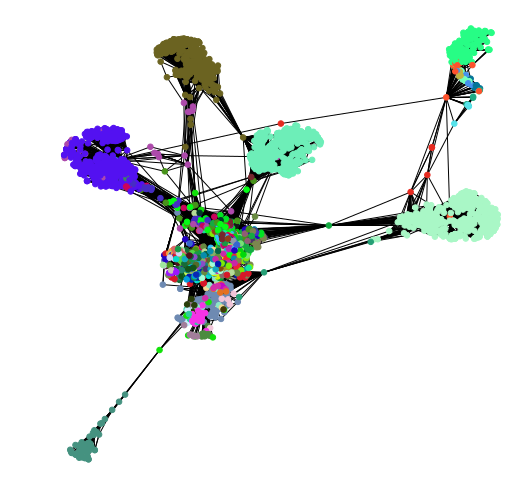
\includegraphics[width=\linewidth]{Chapter3/Chapter3Figs/facebook_demo}
		\caption{Mô phỏng phát hiện cồng đồng trên mạng facebook \ref{testgraphformethod}}
		\label{fig:facebook-demo}
	\end{minipage}
	\begin{minipage}[t]{0.48\textwidth}
		\centering
		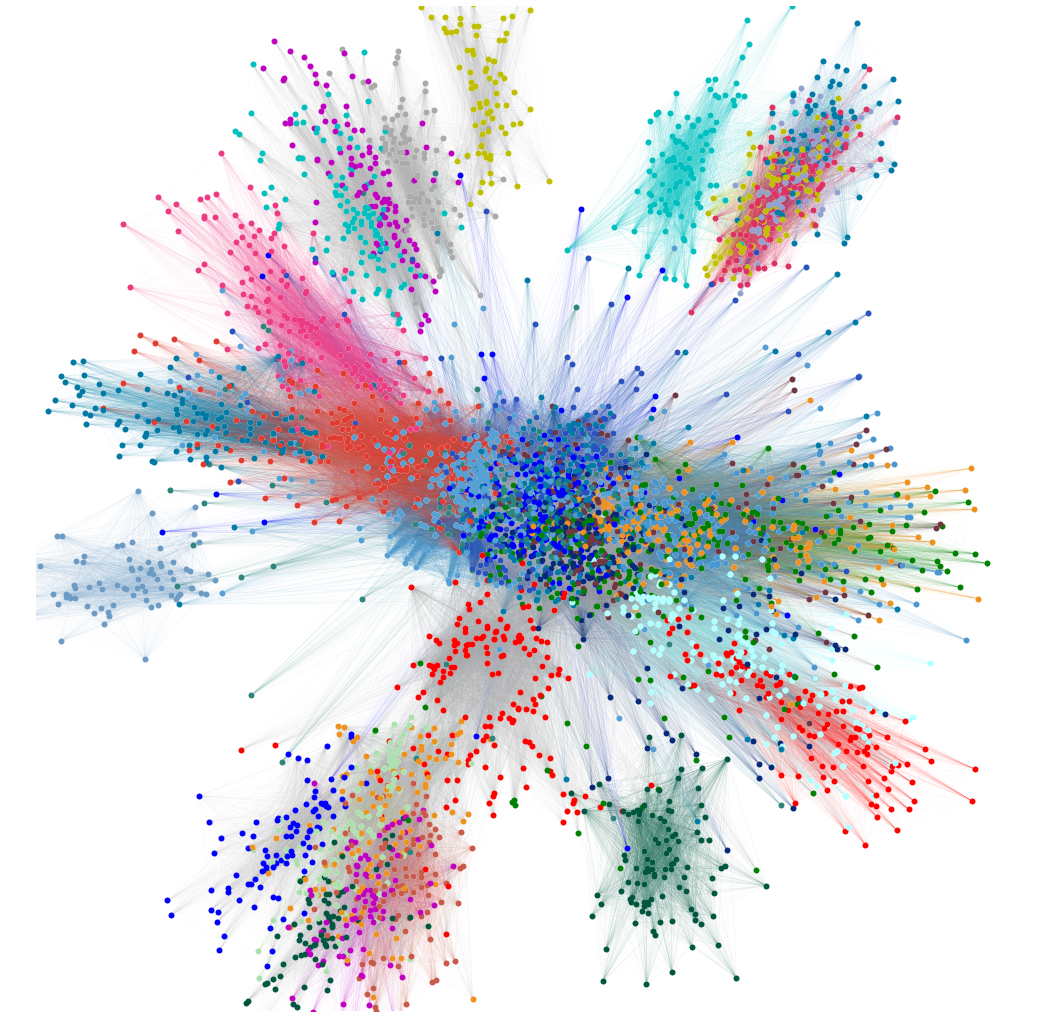
\includegraphics[width=0.7\linewidth]{Chapter3/Chapter3Figs/graph}
		\caption{Mô phỏng phát hiện cồng đồng trên mạng internet \ref{testgraphformethod}}
		\label{fig:graph3}
	\end{minipage}    
\end{figure}

Ngoài ra, việc sử dụng một vài khái niệm sau đã cải thiện hiệu năng đáng kể:
\begin{itemize}
	\item Biến broadcast: được tạo ra bằng cách gọi hàm SparkContext.broadcast(v). Broadcast variable là một wrapper xung quanh biến v, giá trị của biến này có thể được truy xuất thông qua hàm value. Về cơ bản biến broadcast sẽ được phân tán biến biến local trên tất cả các máy worker, điều này làm giảm thời gian cho các máy worker quay trở lại máy master để lấy giá trị.
	\item Biến accumulator: Khi ta muốn thực hiện các thao tác trên tập dữ liệu được phân tán mà không thể thông qua các thao tác RDD hỗ trợ thì biến accumulator cho phép là một biến trung gian (toàn cục) giữa các máy trong cụm. 
	\item phương thức cache/ persist: Cho phép dữ liệu được lưu trữ trên RAM. Điều này giúp cho các tác vụ được sử dụng nhiều lần sẽ có thời gian truy vấn nhanh hơn do dữ liệu đã lưu lại trên RAM.
\end{itemize}

Để quá trình huấn luyện theo công thức \ref{eq:ctfu_hat} trên hệ thống phân phán phát huy tính hiệu quả. Tôi đã đề xuất sử dụng phương pháp tăng gradient ngẫu nhiên theo cụm đã được trình bày trong thuật toán \ref{alg:MBSGD}.
	\def\baselinestretch{1}
\chapter{Kết luận và hướng phát triển}
\ifpdf
    \graphicspath{{Conclusions/ConclusionsFigs/PNG/}{Conclusions/ConclusionsFigs/PDF/}{Conclusions/ConclusionsFigs/}}
\else
    \graphicspath{{Conclusions/ConclusionsFigs/EPS/}{Conclusions/ConclusionsFigs/}}
\fi

\def\baselinestretch{1.66}

\section{Kết luận}
Khóa luận này tập trung làm rõ bài toán phát hiện cộng đồng, đặc biệt với những cộng đồng có tính chồng chéo, lồng nhau. Đồng thời nhấn mạnh mức độ quan trọng của bài toán trong thực tế hiện nay, khi mà các mạng ngày càng trở lên mở rộng cả về cấu trúc lẫn nội dung có thể thấy một ví dụ điểm hình mạng xã hội Facebook với dân số gần $2$ tỷ người được ví như là một quốc gia ảo. 

Nội dung chính của khóa luận là làm rõ mô hình BigCLAM, từ đó đề xuất sử dụng một vài phương pháp tối ưu hàm lồi trong phần \ref{muc:toiuuhamloi} cũng như phương pháp khởi tạo matrix trọng số giúp cho quá trình phát hiện hiệu quả và nhanh hơn.

Đặc biệt, phần chính của khóa luận này hướng đến là cài đặc thực nghiệm phương pháp phát hiện cộng đồng trên cụm máy tính sử dụng hai framework Apache Hadoop trong việc lưu trữ phân tán và Apache Spark trong quá trình tính toán phân tán. Việc chuyển từ bài toán chạy trên một máy sang bài toán phân tán ra nhiều máy là một bài toán không hề dễ dàng nhưng hiệu quả của nó mang lại rất lớn khi mà dữ liệu ngày một lớn và không ngừng tăng trưởng. Lợi thế của hệ thống phân tán là có thể mở rộng tính toán theo chiều ngang vậy nên tôi đã đề xuất phương pháp giảm gradient ngẫu nhiên theo cụm (MBSGD) được trình bày trong thuật toán \ref{alg:MBSGD}. Tuy nhiên, trong quá trình thực nghiệm những dữ liệu lớn hơn khoảng vài triệu đỉnh và cặp cạnh lại cho thấy thời gian khá chậm với nhu cầu thực tế. Điều này cần phải được nghiên cứu kỹ hơn cả về kiến trúc hạ tầng lẫn tối ưu quá trình lập trình phân tán.

Kết luận, khóa luận về cơ bản đã hoàn thành mục tiêu đã đề ra từ đầu trong việc giải quyết bài toán phát hiện cộng đồng trọng mạng tương tác có kích thước lớn. Tuy nhiên, để áp dụng thuật toán vào thực tế cần phải được đầu tư nghiêm túc để phát huy sức mạnh của thuật toán và hệ tính toán phân tán.

\section{Hướng phát triển}
Từ những kết luận trên, trong thời gian tới, tôi sẽ tiếp tục nghiên cứu cải tiến tốc độ bài toán phù hợp với nhu cầu phân tích thời gian thực trên các mạng hiện nay. Đồng thời đưa phương pháp này vào các ứng dụng thực tế. Cụ thể là bài toán xây dựng hệ khuyến nghị trong mạng xã hội giáo dục Đại học Thăng Long.
	
	\backmatter
	\bibliographystyle{plain}
	\bibliography{References/references} % References file  
	\appendix
	\renewcommand{\thechapter}{\arabic{chapter}}
	\renewcommand{\thesection}{A.\arabic{section}}
	\label{appendixA}
	\chapter{Phụ lục A:\\ Cài đặt và triển khai ứng dụng trên Apache Hadoop \& Spark}

Tại chương \ref{chap:c4} triển khai phương pháp phát hiện cộng đồng được trình bày ở chương \ref{chap:c3} trên hai framework Apache Hadoop và Apache Spark. Trong chương này, tôi sẽ trình bày các cài đặt và triển khai ứng dụng trên hai framework này.

\section{Cài đặt}
Apache Hadoop và Spark được phát triển trên nền tảng GNU/Linux và hoạt động tốt trên môi trường này. Vì vậy, chúng ta nên sử dụng hệ điều hành Linux để cài đặt hai framework này. Giả sử ta sẽ cài đặt hai framework trên một cụm máy gồm $3$ node (worker) và $1$ node (master).

Đầu tiên, ta cần xác định địa chỉ mạng và thiết đặt địa chỉ tĩnh trên mỗi máy trong cụm. Điều này nhằm cố định địa chỉ mạng trên mỗi máy tính. Ví dụ như sau:
\begin{table}[H]
	\centering
	\caption{Các địa chỉ IP trong cụm}
	\label{ipaddress}
	\begin{tabular}{@{}cll@{}}
		\toprule
		\multicolumn{1}{l}{\textbf{STT}} & \multicolumn{1}{l}{\textbf{Địa chỉ IP}} & \multicolumn{1}{l}{\textbf{Vai trò}} \\ \midrule
		$1$                                & $192.168.100.10$                  & master                               \\
		$2$                                & $192.168.100.11$                  & worker1                              \\
		$3$                               & $192.168.100.12$                  & worker2                              \\
		$4$                                & $192.168.100.13$                  & worker3                              \\ \bottomrule
	\end{tabular}
\end{table}

Bước tiếp theo, ta tiến hành cập nhật file hots (\textit{/etc/hosts}) theo bảng \ref{ipaddress} trên mỗi máy tính. Mục đích là để $4$ node này nó thấy nhau qua tên máy hoặc IP.

Để xác thực giữa các máy trong cụm với nhau nhằm tạo một cơ chế bảo mật và không yêu cầu mật khẩu qua mỗi lần khởi chạy, ta sẽ sử dụng thông qua cơ chế SSH. Để cài đặt SSH ta dùng lệnh:
\begin{quote}
	\textbf{\textit{\$ sudo apt-get install openssh-server openssh-client}}
\end{quote}
Sau đó tiến hành sinh khóa $RSA$ và sao chép khóa publickey cho các máy \textit{worker} (thực hiện trên máy \textit{master}):\\
\begin{quote}
	\textbf{\textit{\$ ssh-keygen\\
	\$ cd $\sim$/.ssh\\
	\$ ssh-copy-id -i id\_rsa.pub sv@worker1\\
	\$ ssh-copy-id -i id\_rsa.pub sv@worker2\\
	\$ ssh-copy-id -i id\_rsa.pub sv@worker3\\
	\$ cat id\_rsa.pub $\gg$ authorized\_keys}}
\end{quote}

Sửa tên máy cho đúng với \textit{master} và từng \textit{worker}, chạy lệnh:
\begin{quote}
	\textbf{\textit{\$ hostnamectl set-hostname master\\
			\$ hostnamectl set-hostname worker1 \\
			\$ hostnamectl set-hostname worker2 \\
			\$ hostnamectl set-hostname worker3}}
\end{quote}
\subsection{Apache Hadoop \& Spark}
Tiến hành tải và cài đặt các gói cài đặt Java, Scala, Apache Hadoop, Apache Spark (Chú ý chọn các phiên bản java, scala hỗ trợ hadoop và spark).
e\begin{itemize}
	\item \textbf{Scala:} http://www.scala-lang.org/download/
	\item \textbf{Java:} https://www.java.com/en/download/
	\item \textbf{Apache Hadoop:} http://hadoop.apache.org/releases.html
	\item \textbf{Apache Spark:} http://spark.apache.org/downloads.html
\end{itemize}

Tại thời điểm thực hiện đề tài, tôi sử dụng các phiên bản sau:
\begin{table}[H]
	\centering
	\caption{Các phiên bản cài đặt}
	\label{versionlist}
	\begin{tabular}{@{}cll@{}}
		\toprule
		\multicolumn{1}{l}{STT} & Gói cài đặt   & Phiên bản                     \\ \midrule
		$1$                     & Scala         & scala-2.12.1.tgz              \\
		$2$                     & Java          & jdk-8u121-linux-x64.tar.gz    \\
		$3$                     & Apache Hadoop & hadoop-2.7.2.tar.gz           \\
		$4$                     & Apache Spark  & spark-2.1.0-bin-hadoop2.7.tgz \\ \bottomrule
	\end{tabular}
\end{table}

Tiến hành giải nén và chuyển vào mục cài đặt các gói cài đặt:
\begin{quote}
	\textbf{\textit{// Giải nén gói cài đặt \\
	\$ tar -xvf jdk-8u121-linux-x64.tar.gz \\
	\$ tar -xvf hadoop-2.7.2.tar.gz \\
	\$ tar -xvf spark-2.1.0-bin-hadoop2.7.tgz \\
	\$ tar -xvf scala-2.12.1.tgz \\
	// Tạo thư mục cài đặt \\
	\$ sudo mkdir /usr/local/java \\
	\$ sudo mkdir /usr/local/hadoop \\
	\$ sudo mkdir /usr/local/spark \\
	\$ sudo mkdir /usr/local/scala \\
	// Chuyển file cài đặt vào thư mục cài đặt \\
	\$ sudo mv jdk1.8.0\_121 /usr/local/java/jdk1.8.0\_121  \\
	\$ sudo mv hadoop-2.7.2 /usr/local/hadoop/2.7.2 \\
	\$ sudo mv spark-2.1.0-bin-hadoop2.7 \\ /usr/local/spark/2.1.0 \\
	\$ sudo mv scala-2.12.1 /usr/local/scala/scala-2.12.1  \\}}
\end{quote}

Sau đó ta tiến hành thiết lập (\textit{nano $\sim$/.bashrc}) và cập nhật môi trường(\textit{source $\sim$/.bashrc}) như sau:
\begin{quote}
	export JAVA\_HOME=/usr/local/java/jdk1.8.0\_121\\
	export JRE\_HOME=\$JAVA\_HOME/jre\\
	export SCALA\_HOME=/usr/local/src/scala/scala-2.12.1\\
	export SPARK\_HOME=/usr/local/spark/2.1.0\\
	export HADOOP\_HOME=/usr/local/hadoop/2.7.2\\	export PATH=\$PATH:\$JAVA\_HOME/bin:\$JRE\_HOME/bin:\$SCALA\_HOME/bin:\\
	\$SPARK\_HOME/bin:\$SPARK\_HOME/sbin:\\
	\$HADOOP\_HOME/bin:\$HADOOP\_HOME/sbin
\end{quote}
\subsection{Cấu hình Hadoop}
Cấu hình danh sách các máy làm \textit{master}:
\begin{quote}
	\textbf{\textit{\$ nano \$HADOOP\_HOME/etc/hadoop/masters}}
\end{quote}

Cấu hình danh sách các máy làm \textit{worker}:
\begin{quote}
	\textbf{\textit{\$ nano \$HADOOP\_HOME/etc/hadoop/slaves}}
\end{quote}

Khởi tạo namenode cho máy master
\begin{quote}
	\textbf{\textit{\$ mkdir -p
	\$ \$HADOOP\_HOME/hadoop\_store/hdfs/namenode}}
\end{quote}
Khởi tạo datanode cho máy worker
\begin{quote}
	\textbf{\textit{\$ mkdir -p \$HADOOP\_HOME/hadoop\_store/hdfs/datanode\\
	\$ chmod 755 \$HADOOP\_HOME/hadoop\_store/hdfs/datanode}}
\end{quote}
Cấu hình core-site.xml:
\begin{quote}
	<property>\\
		<name>fs.defaultFS</name>\\
		<value>hdfs://master:8020</value>\\
	</property>
\end{quote}
Cấu hình hdfs-site.xml:
\begin{quote}
	<property>\\
	<name>dfs.namenode.name.dir</name>\\
	<value>file:/usr/local/hadoop/2.7.2/hadoop\_store/hdfs/namenode</value>\\
	</property>\\
	<property>\\
	<name>dfs.datanode.data.dir</name>\\
	<value>file:/usr/local/hadoop/2.7.2/hadoop\_store/hdfs/datanode</value>\\
	</property>\\
	<property>\\
	<name>dfs.replication</name>\\
	<value>3</value>\\
	</property>\\
\end{quote}
Cấu hình mapred-site.xml:
\begin{quote}
	<property>\\
	<name>mapreduce.framework.name</name>\\
	<value>yarn</value>\\
	</property>
\end{quote}
Cấu hình yarn-site.xml:
\begin{quote}
	<property>\\
	<name>yarn.resourcemanager.resource-tracker.address</name>\\
	<value>master:8025</value>\\
	</property>\\
	<property>\\
	<name>yarn.resourcemanager.scheduler.address</name>\\
	<value>master:8030</value>\\
	</property>\\
	<property>\\
	<name>yarn.resourcemanager.address</name>\\
	<value>master:8050</value>\\
	</property>\\
	<property>\\
	<name>yarn.nodemanager.aux-services</name>\\
	<value>mapreduce\_shuffle</value>\\
	</property>\\
	<property>\\
	<name>yarn.nodemanager.aux-services.mapreduce.shuffle.class</name>\\
	<value>org.apache.hadoop.mapred.ShuffleHandler</value>\\
	</property>\\
	<property>\\
	<name>yarn.nodemanager.disk-health-checker.min-healthy-disks</name>\\
	<value>0</value>\\
	</property>
	
\end{quote}

Tiến hành định dạng HDFS:
\begin{quote}
	\textbf{\textit{\$ \$HADOOP\_HOME/bin/hdfs namenode -format}}
\end{quote}

\subsection{Cấu hình Spark}
Cấu hình danh sách các máy làm \textit{worker}:
\begin{quote}
	\textbf{\textit{\$ nano \$SPARK\_HOME/conf/slaves}}
\end{quote}
Cấu hình spark-env.sh:
\begin{quote}
	SPARK\_WORKER\_MEMORY=1g\\
	SPARK\_WORKER\_INSTANCES=1\\
	SPARK\_WORKER\_CORES=2\\
	SPARK\_MASTER\_HOST=master\\
	HADOOP\_CONF\_DIR=/usr/local/hadoop/2.7.2/etc/hadoop
\end{quote}
Cấu hình spark-defaults.sh:
\begin{quote}
	spark.master                     spark://192.168.100.10:7077
\end{quote}

\section{Tập lệnh}
\subsection{Danh sách tập lệnh làm việc trên Hadoop}
\begin{table}[H]
	\centering
	\caption{Danh sách tập lệnh cơ bản làm việc trên Hadoop}
	\label{my-hadoop}
	\begin{tabular}{@{}lll@{}}
		\toprule
		STT                     & Lệnh                                                & Ý nghĩa                             \\ \midrule
		$1$ & hadoop namenode -format                             & format hdfs                         \\
		$2$ & \$HADOOP\_HOME/sbin/start-dfs.sh                    & Khởi động hdfs: http://master:50070 \\
		$3$ & \$HADOOP\_HOME/sbin/start-yarn.sh                   & Khởi động yarn: http://master:8088  \\
		$4$ & \$HADOOP\_HOME/sbin/stop-dfs.sh                     & Dừng hdfs                           \\ 
		$5$                     & \$HADOOP\_HOME/sbin/start-yarn.sh                   & Dừng yarn                           \\
		$6$                     & \$HADOOP\_HOME/sbin/start-all.sh                    & Khởi động hdfs + yarn               \\
		$7$                     & \$HADOOP\_HOME/sbin/stop-all.sh                     & Dừng hdfs + yarn                    \\
		$8$                     & \$HADOOP\_HOME/sbin/hadoop-daemon.sh start datanode & Khởi động trên máy worker           \\
		$9$                     & hadoop fs -mkdir -p /Documents/Data                 & Tạo floder Data trên HDFS           \\
		$10$                    & hadoop fs -rm /Documents/Data/datatest.txt          & Xóa file Data trên HDFS             \\
		$11$                    & hadoop fs -rmdir /user/output                       & Xóa floder Data trên HDFS           \\
		$12$                    & hadoop fs -ls /user/output                          & Liệt kê file trên HDFS              \\
		$13$                    & hadoop fs -cat /user/output/NTMerged.txt     & Hiển thị nội dung file              \\
		$14$                    & hadoop fs -cat data.txt /Document/Data/             & Đẩy file local lên HDFS            
	\end{tabular}
\end{table}
\subsection{Danh sách tập lệnh làm việc trên Spark}
\begin{table}[H]
	\centering
	\caption{Danh sách tập lệnh cơ bản làm việc trên Spark}
	\label{my-spark}
	\begin{tabular}{@{}cll@{}}
		\toprule
		\multicolumn{1}{l}{STT} & Lệnh                            & Ý nghĩa                                    \\ \midrule
		$1$                     & \$SPARK\_HOME/sbin/start-all.sh & Khởi động Spark                            \\
		$2$                     & \$SPARK\_HOME/sbin/stop-all.sh  & Dừng Spark                                 \\
		$3$                     & \$SPARK\_HOME/bin/spark-shell   & Lập trình ứng dụng sử dụng ngôn ngữ scala  \\
		$4$                     & \$SPARK\_HOME/bin/pyspark       & Lập trình ứng dụng sử dụng ngôn ngữ python \\
		$5$ & \$SPARK\_HOME/bin/sparkR        & Lập trình ứng dụng sử dụng ngôn ngữ R      \\
		$6$ & \$SPARK\_HOME/bin/spark-submit  & Tạo ứng dụng                               \\ \bottomrule
	\end{tabular}
\end{table}
% ------------------------------------------------------------------------

%%% Local Variables: 
%%% mode: latex
%%% TeX-master: "../thesis"
%%% End: 

	%\bibliographystyle{plainnat}
	%\bibliographystyle{Classes/jmb} % bibliography style
	%\renewcommand{\bibname}{References} % changes default name Bibliography to References
	
	
\end{document}
